\begin{apendicesenv}

\chapter{Visualização dos resultados globais}
\label{Visualização dos resultados globais}

A Figura~\ref{fig:acc} apresenta a acurácia das arquiteturas avaliadas.  
As Figuras~\ref{fig:f1-normal} e \ref{fig:f1-anormal} exibem, respectivamente, os valores de \textit{F1-score} para as classes Normal e Anormal.

As Figuras~\ref{fig:prec-normal} e \ref{fig:prec-anormal} mostram a precisão das duas classes, enquanto as Figuras~\ref{fig:rec-normal} e \ref{fig:rec-anormal} apresentam os respectivos valores de \textit{recall}.

Por fim, as Figuras~\ref{fig:f1_macro} a \ref{fig:prec_ponderado} reúnem as métricas macro e ponderadas, permitindo uma visão consolidada do desempenho global.

% ---------------- FIGURAS ----------------

\begin{figure}[!h]
    \caption{Acurácia para todas as arquiteturas}
    \centering
    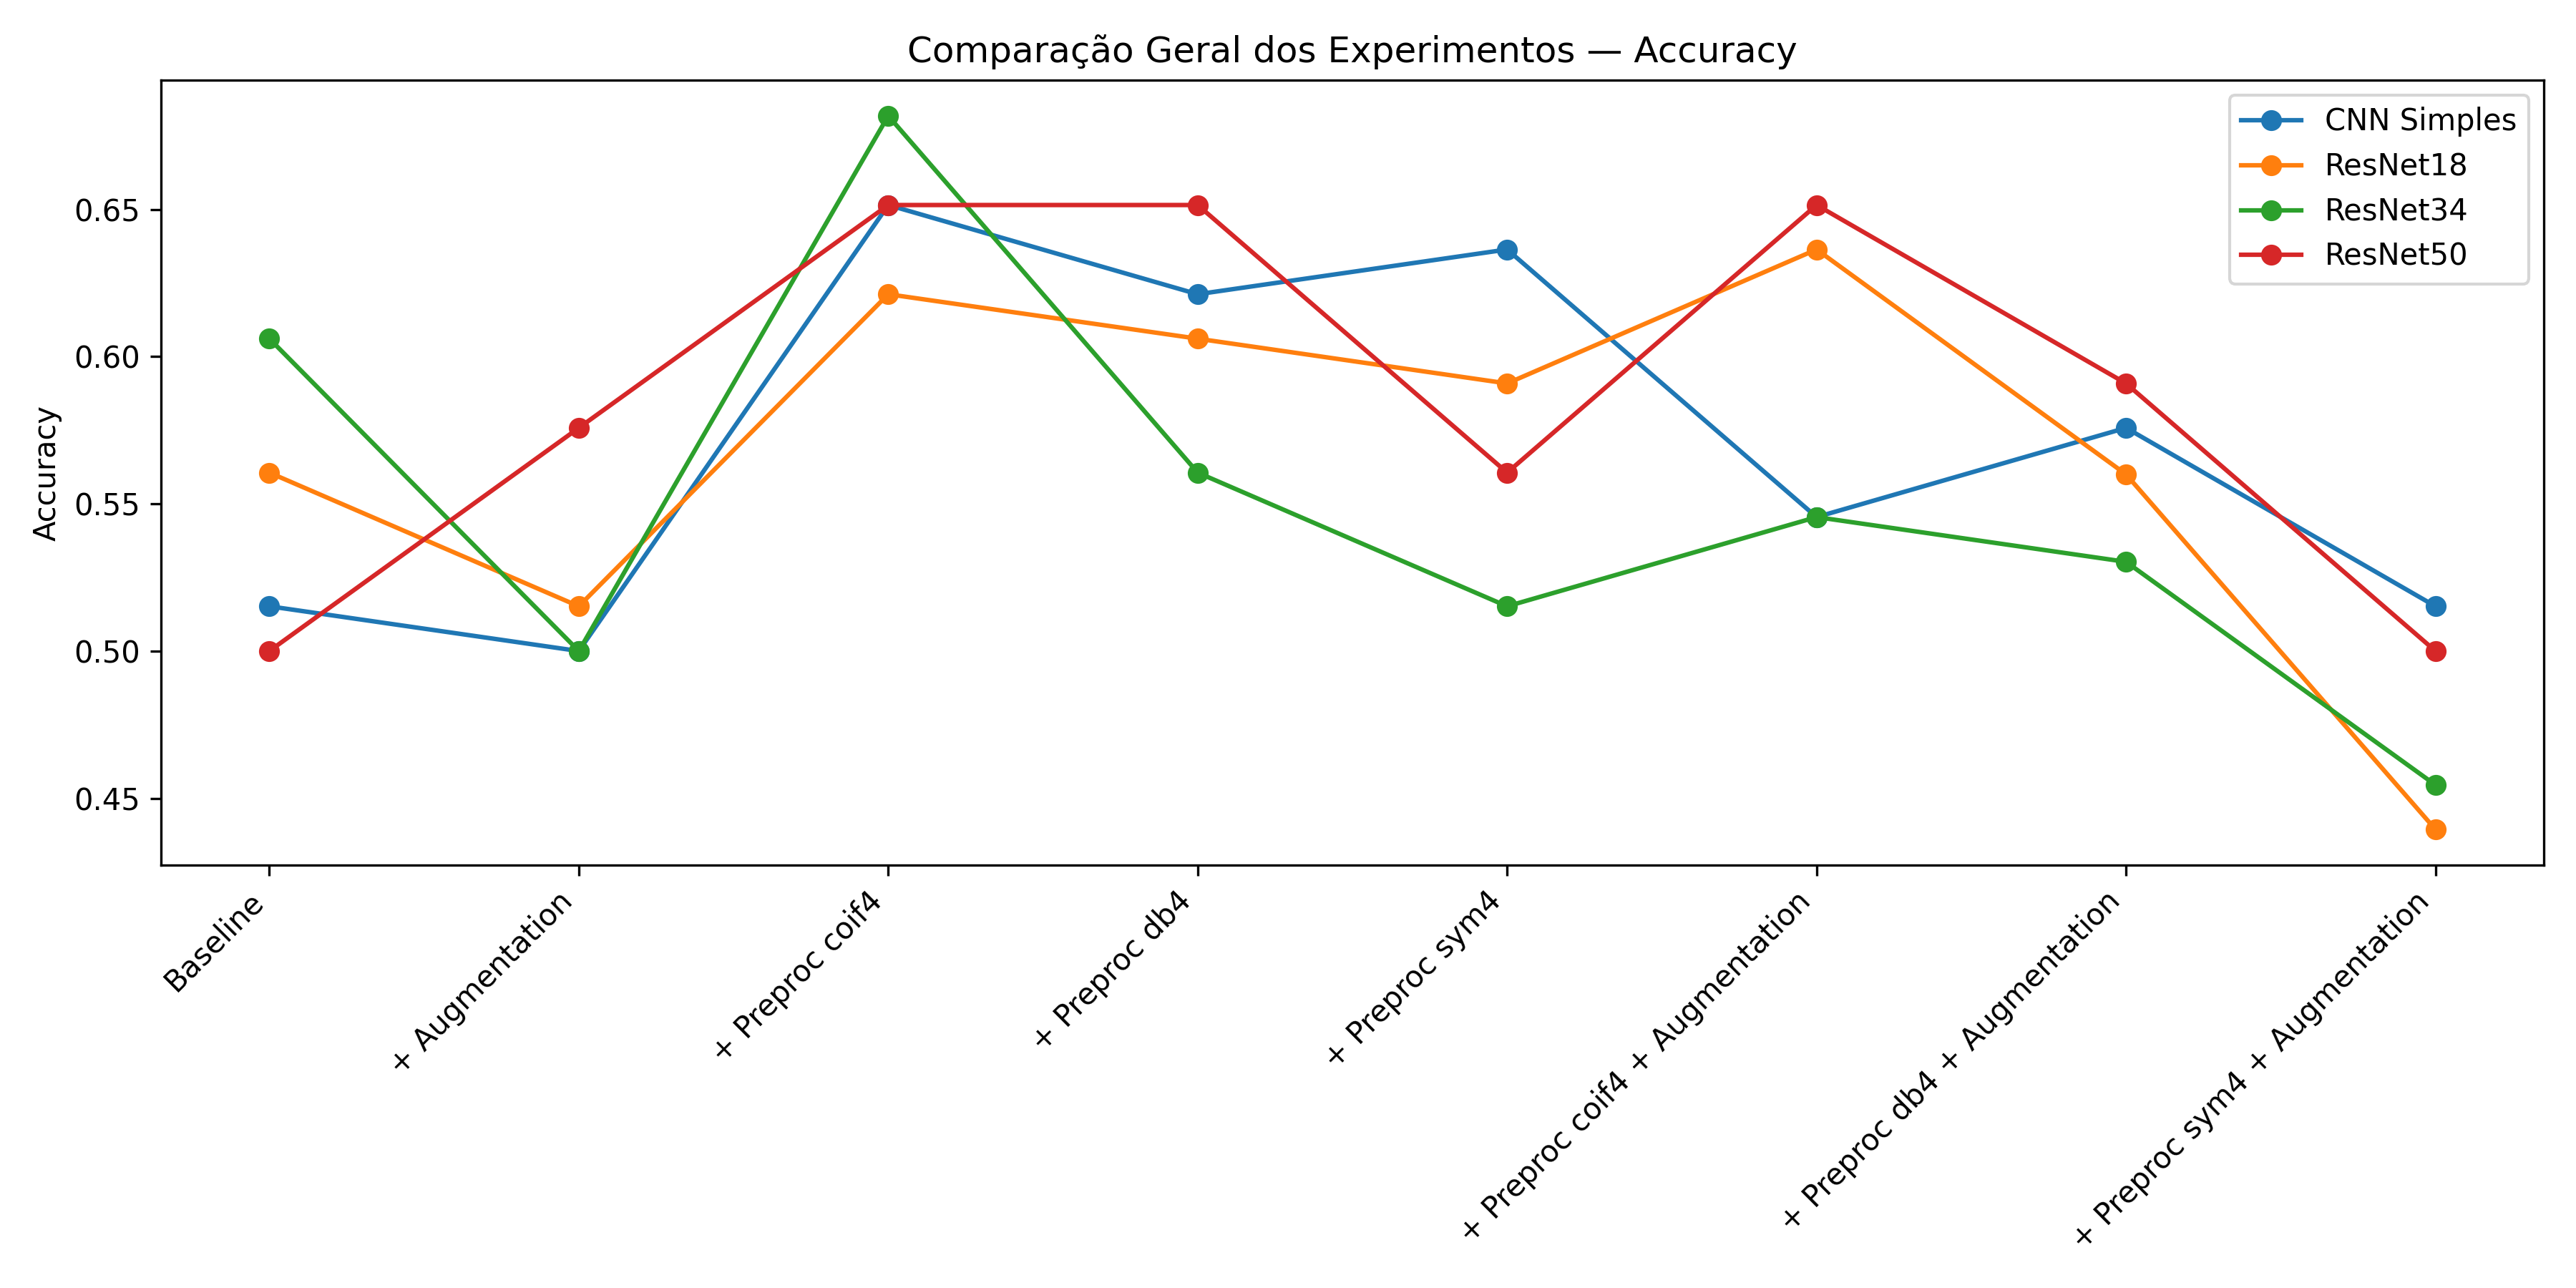
\includegraphics[width=\textwidth]{figuras/GERAL_Accuracy.png}
    \label{fig:acc}
    \fonteproprioautor
\end{figure}

\begin{figure}[!h]
    \caption{F1-score - Classe Normal}
    \centering
    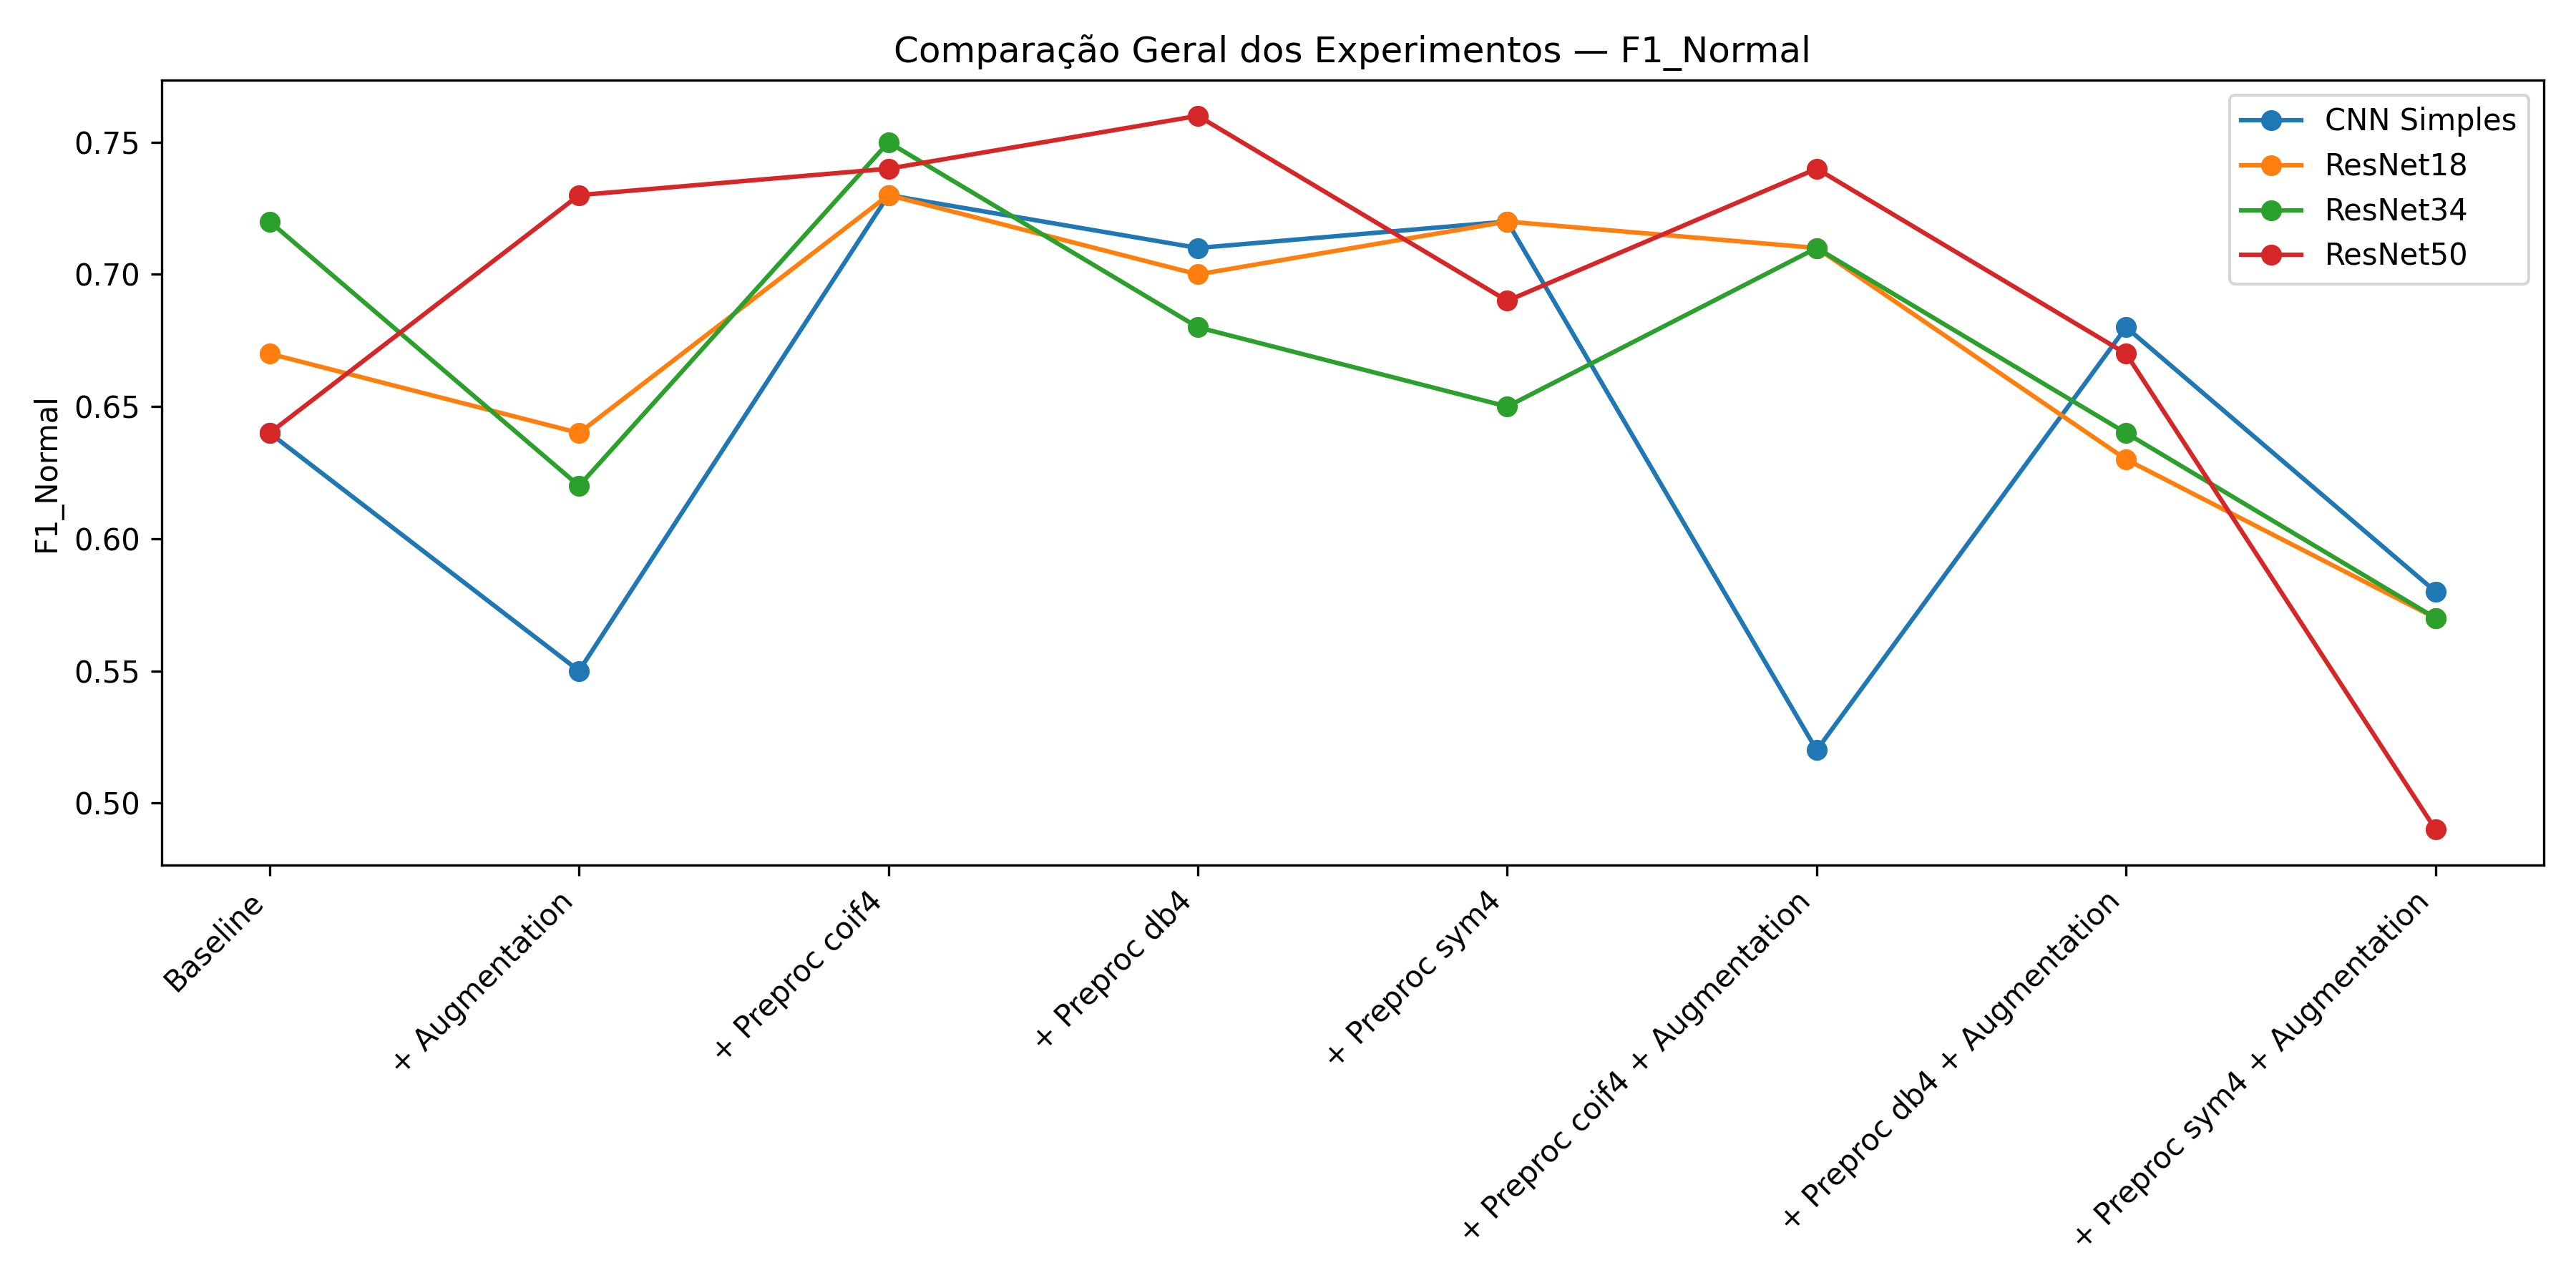
\includegraphics[width=\textwidth]{figuras/GERAL_F1_Normal.png}
    \label{fig:f1-normal}
    \fonteproprioautor
\end{figure}

\begin{figure}[!h]
    \caption{F1-score - Classe Anormal}
    \centering
    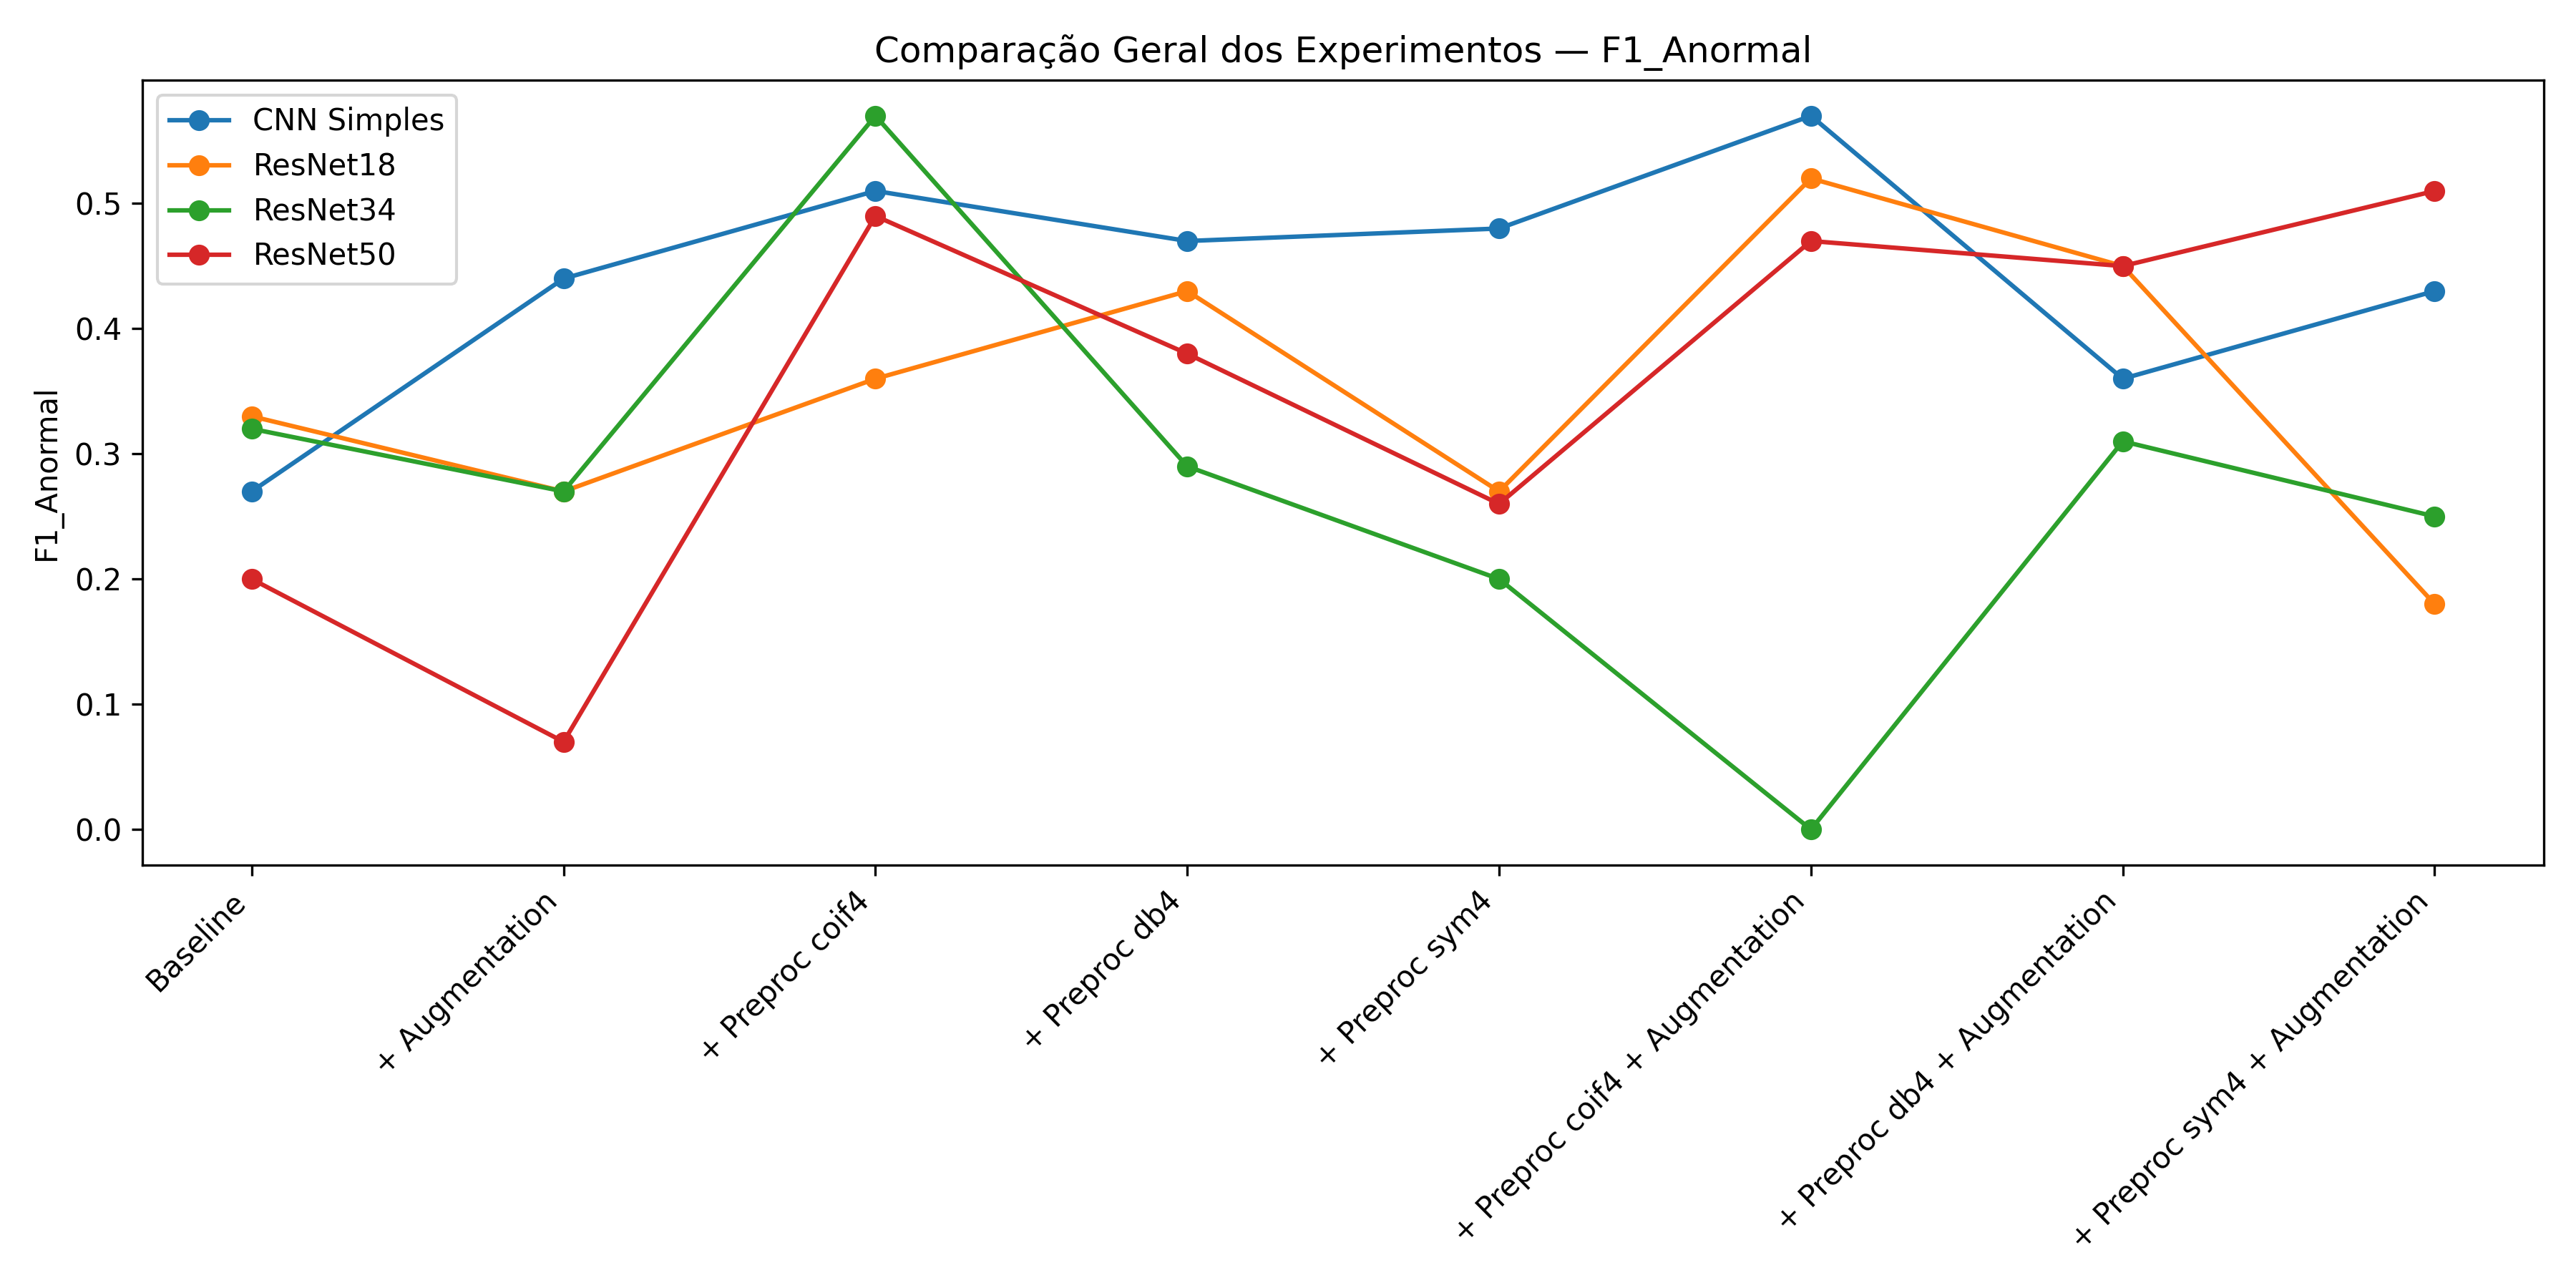
\includegraphics[width=\textwidth]{figuras/GERAL_F1_Anormal.png}
    \label{fig:f1-anormal}
    \fonteproprioautor
\end{figure}

\begin{figure}[!h]
    \caption{Precisão - Classe Normal}
    \centering
    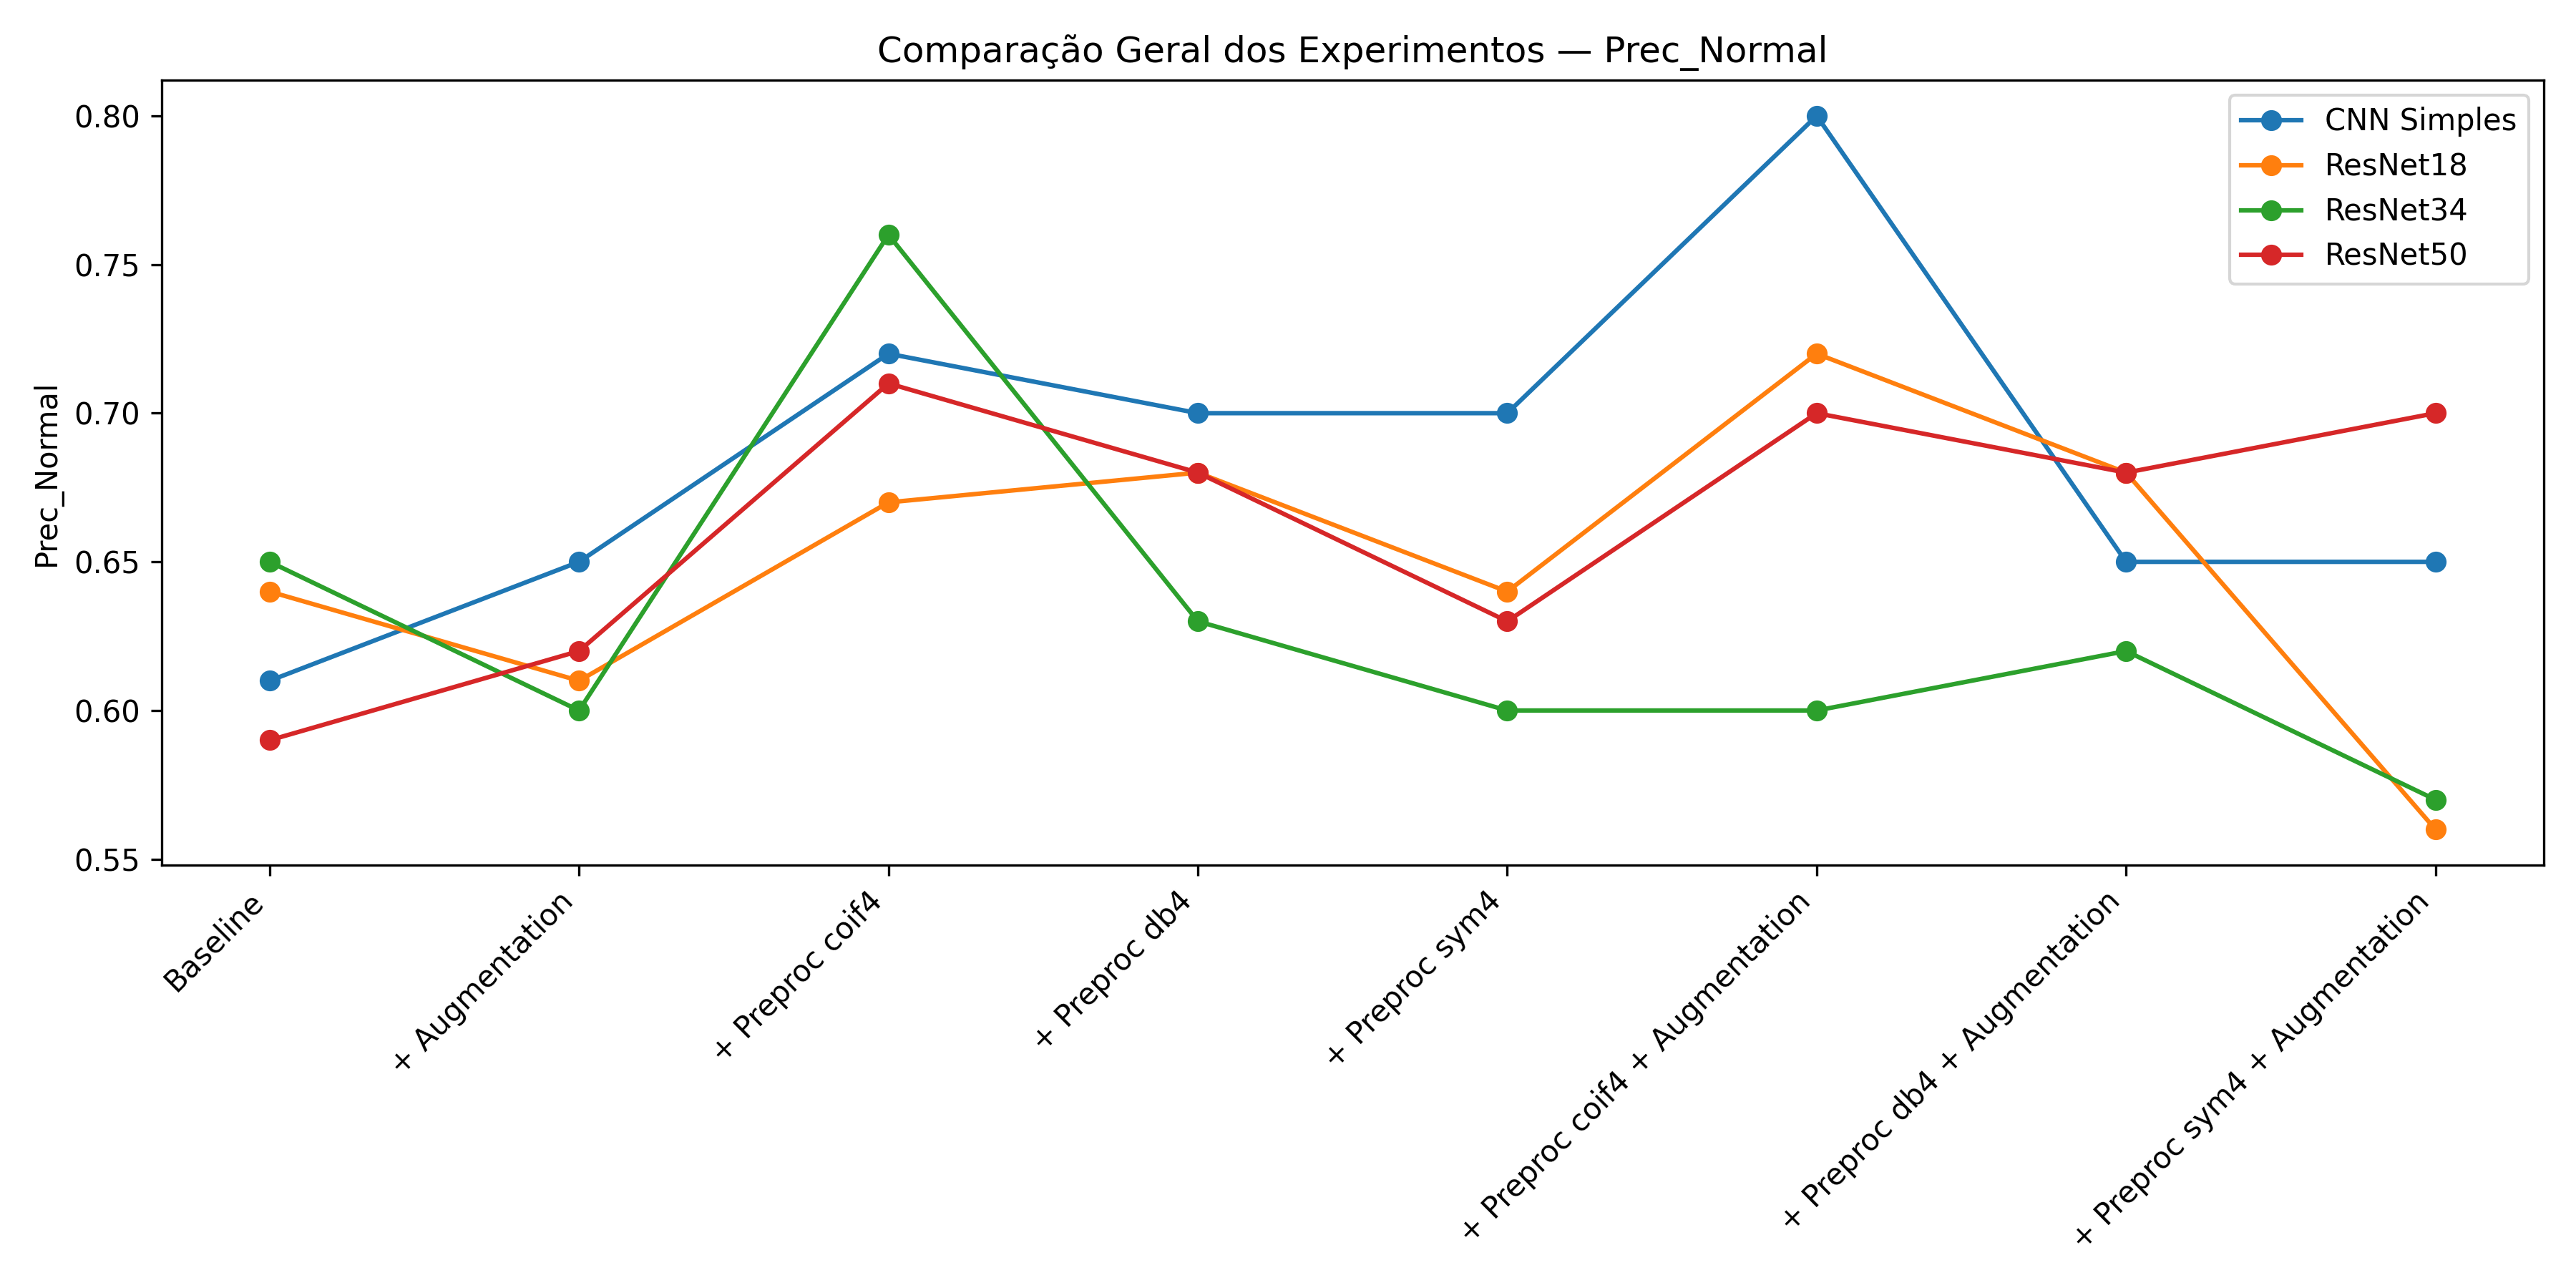
\includegraphics[width=\textwidth]{figuras/GERAL_Prec_Normal.png}
    \label{fig:prec-normal}
    \fonteproprioautor
\end{figure}

\begin{figure}[!h]
    \caption{Precisão - Classe Anormal}
    \centering
    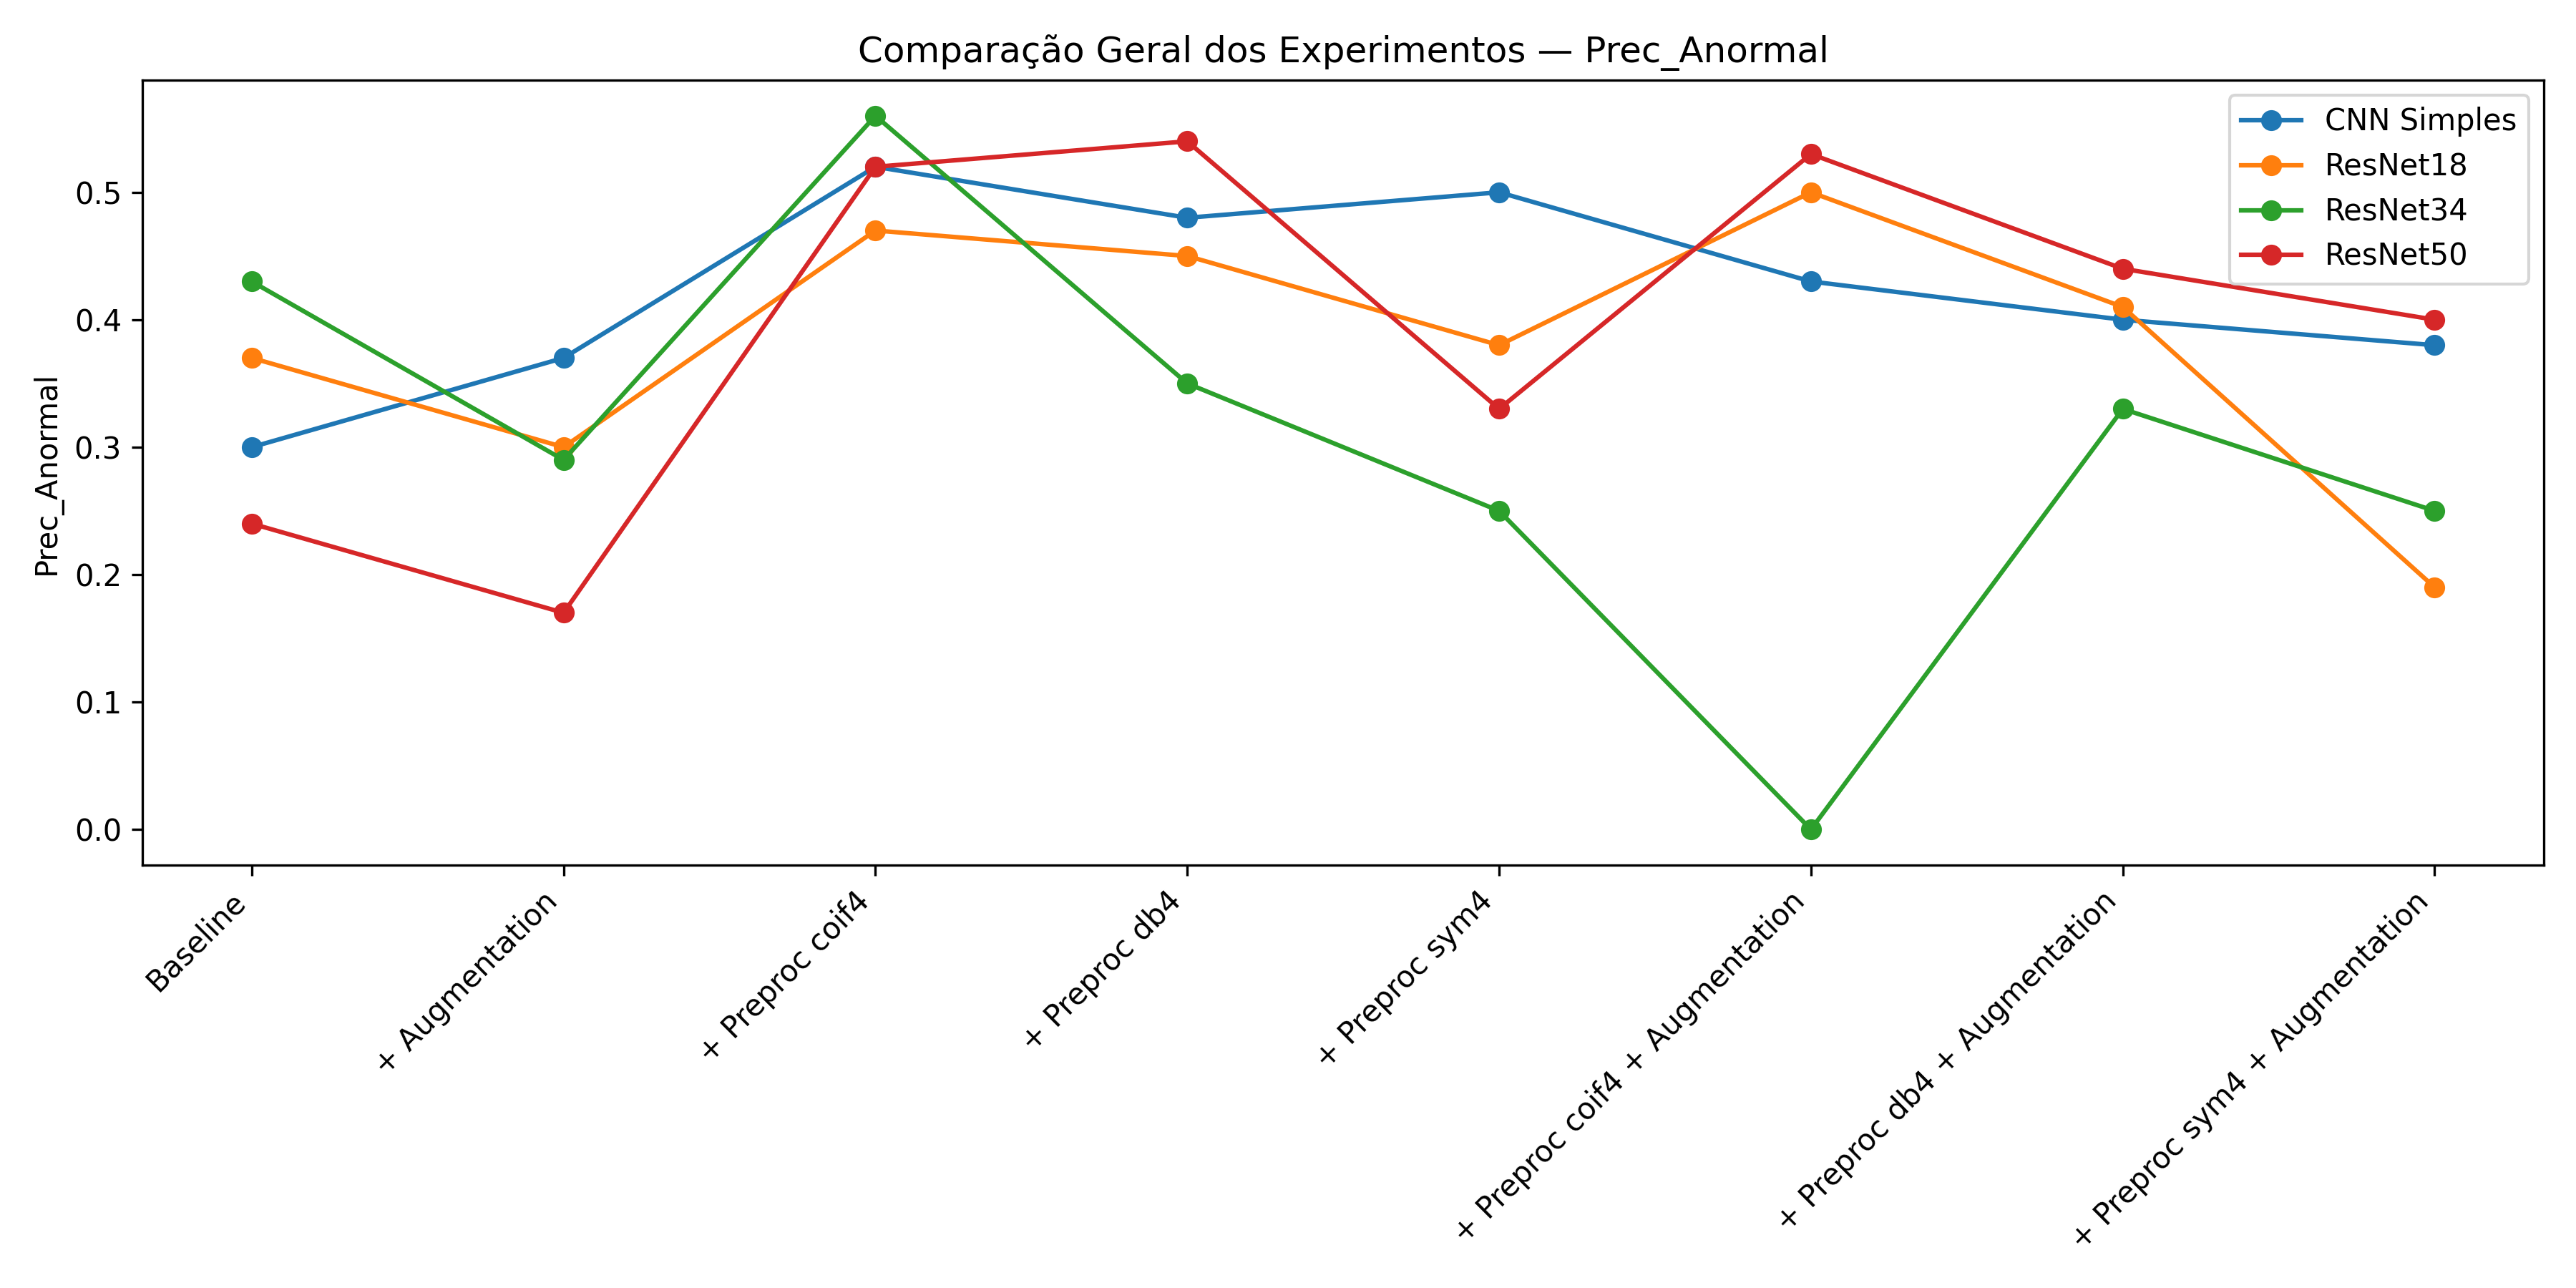
\includegraphics[width=\textwidth]{figuras/GERAL_Prec_Anormal.png}
    \label{fig:prec-anormal}
    \fonteproprioautor
\end{figure}

\begin{figure}[!h]
    \caption{Recall - Classe Normal}
    \centering
    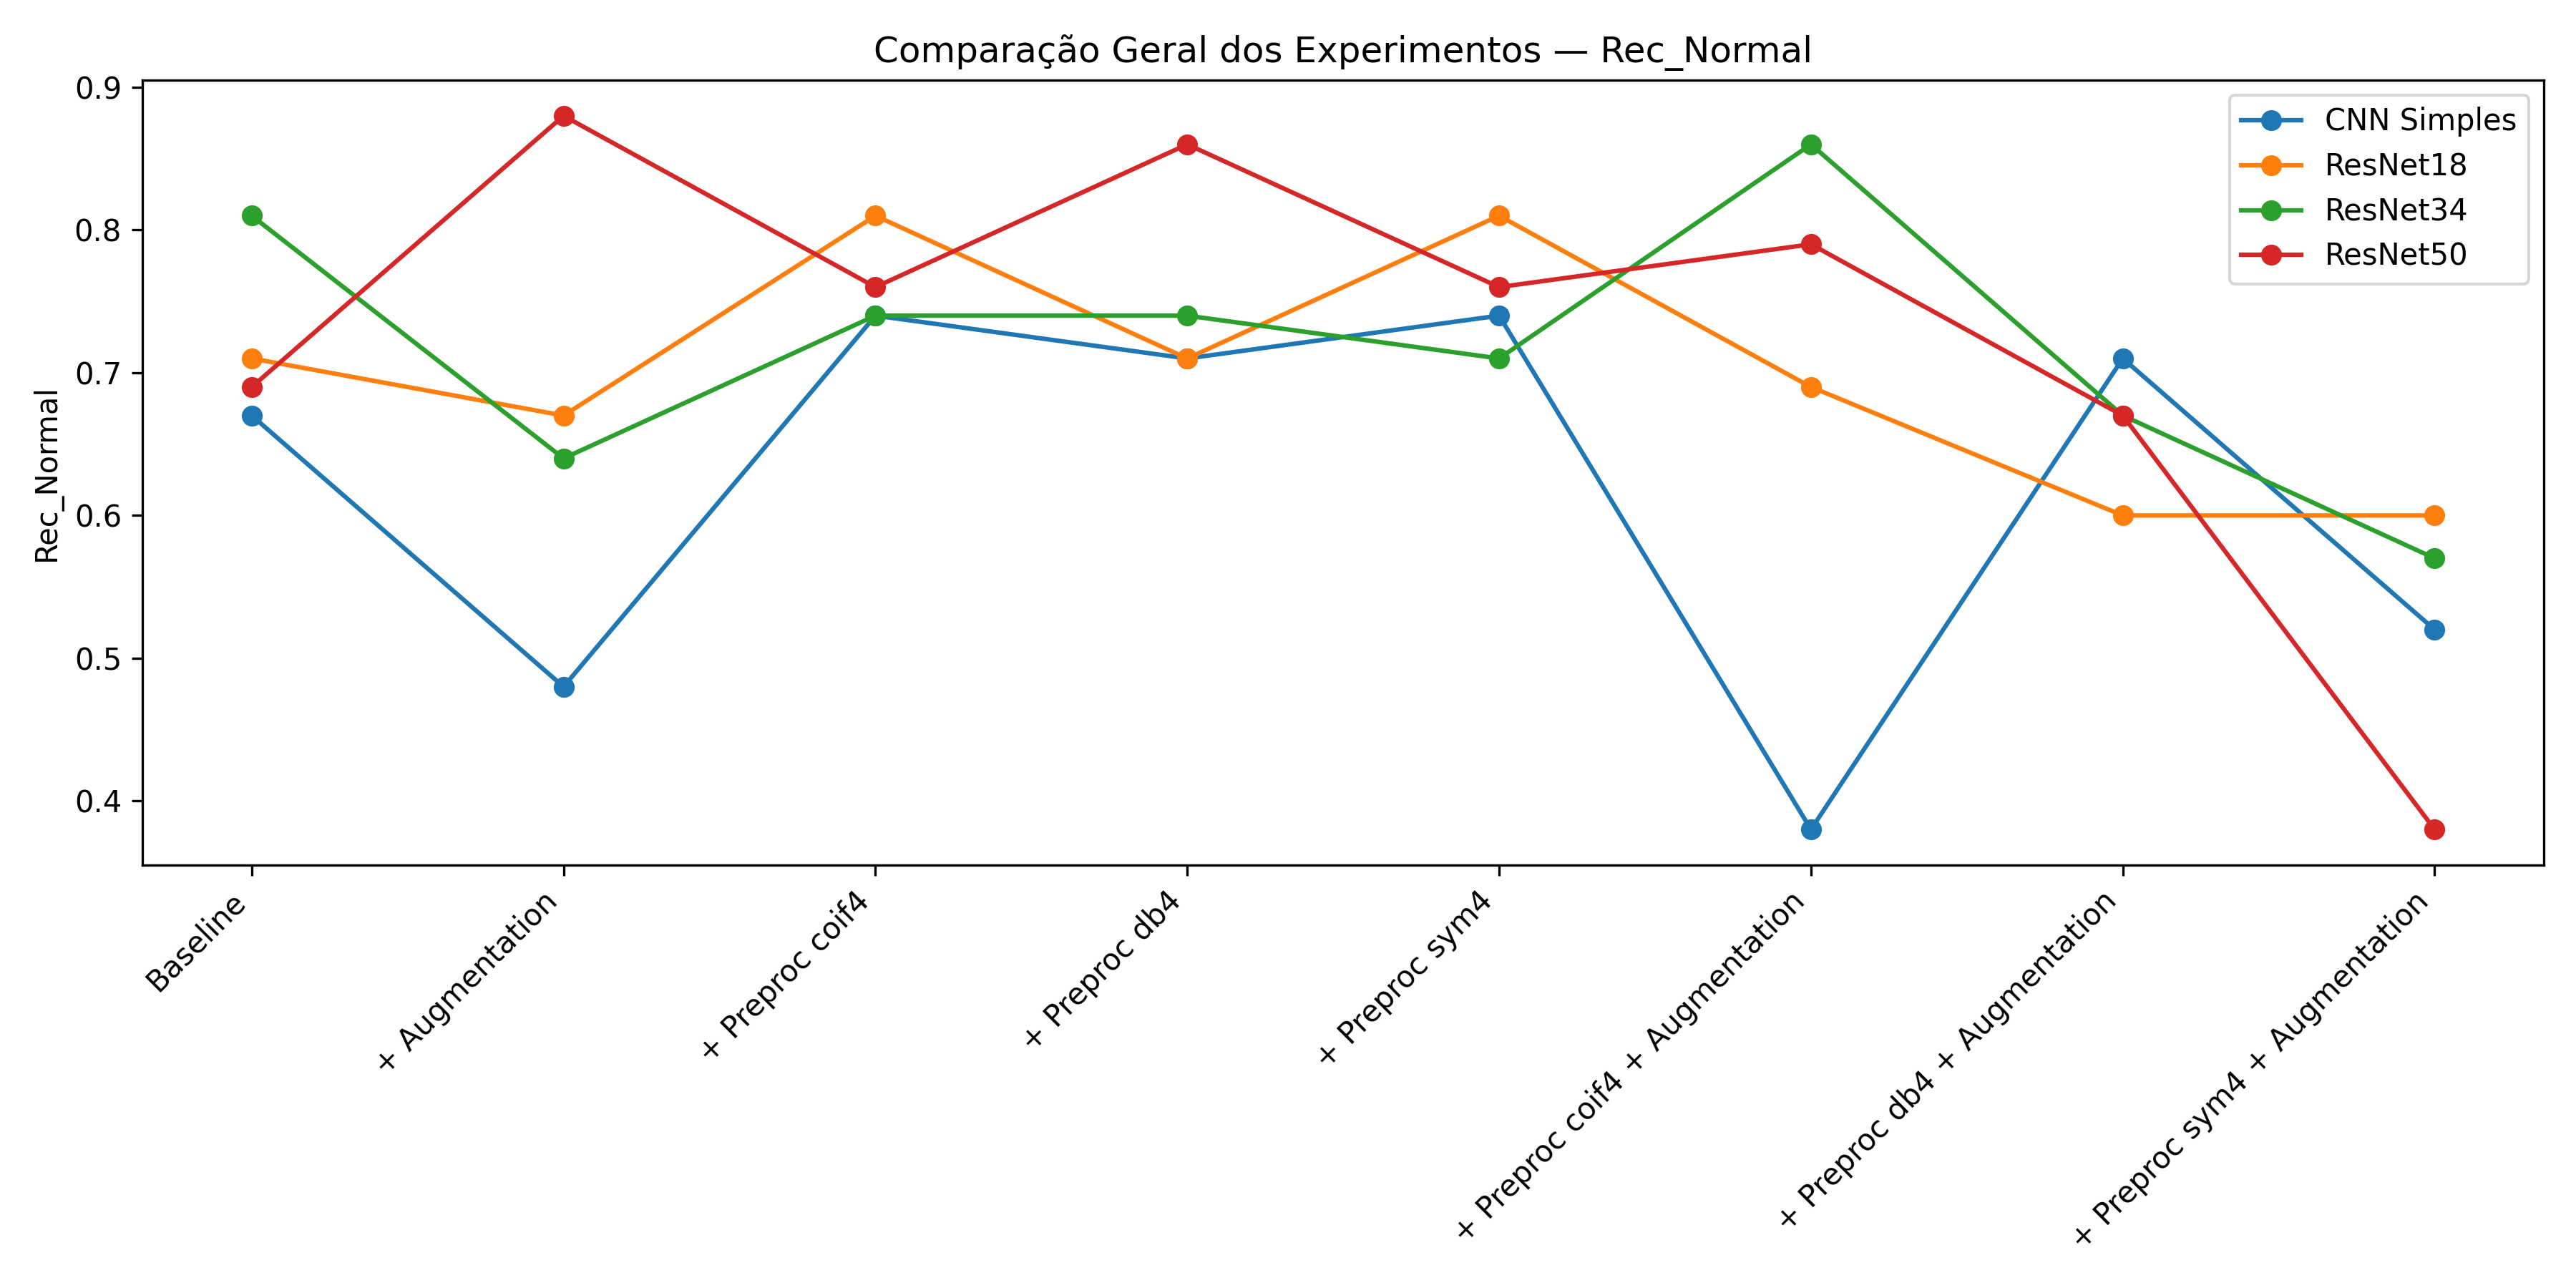
\includegraphics[width=\textwidth]{figuras/GERAL_Rec_Normal.png}
    \label{fig:rec-normal}
    \fonteproprioautor
\end{figure}

\begin{figure}[!h]
    \caption{Recall - Classe Anormal}
    \centering
    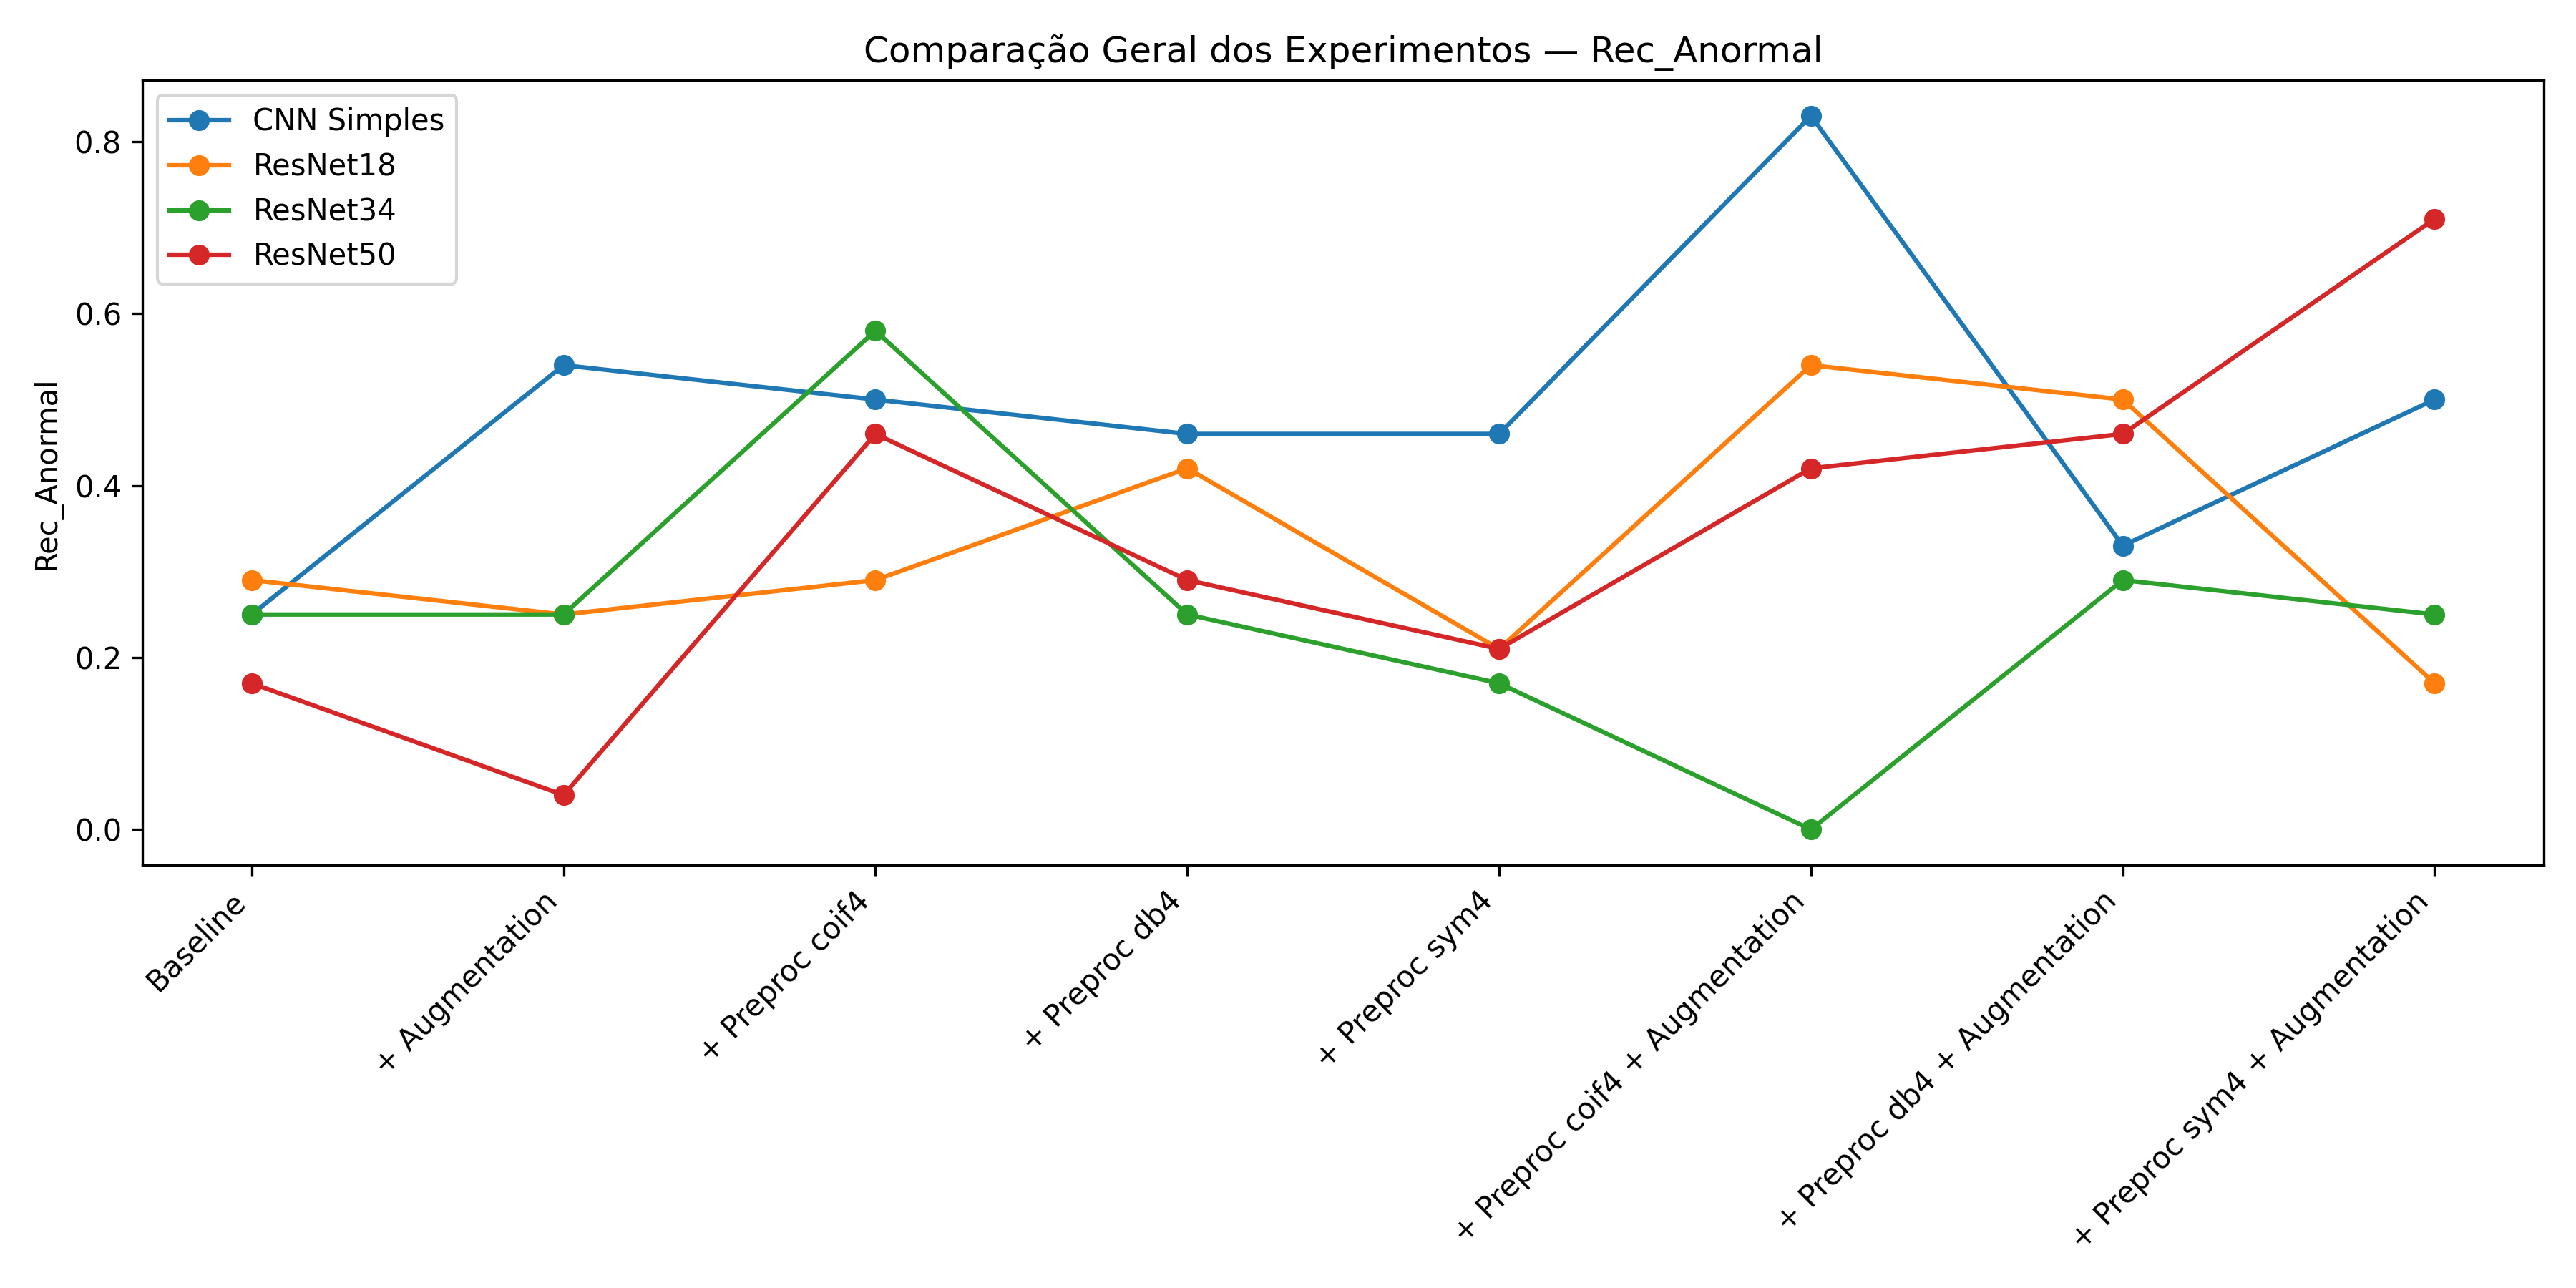
\includegraphics[width=\textwidth]{figuras/GERAL_Rec_Anormal.png}
    \label{fig:rec-anormal}
    \fonteproprioautor
\end{figure}

% Figuras macro e ponderadas 

\begin{figure}[!h]
    \caption{F1-score - Macro}
    \centering
    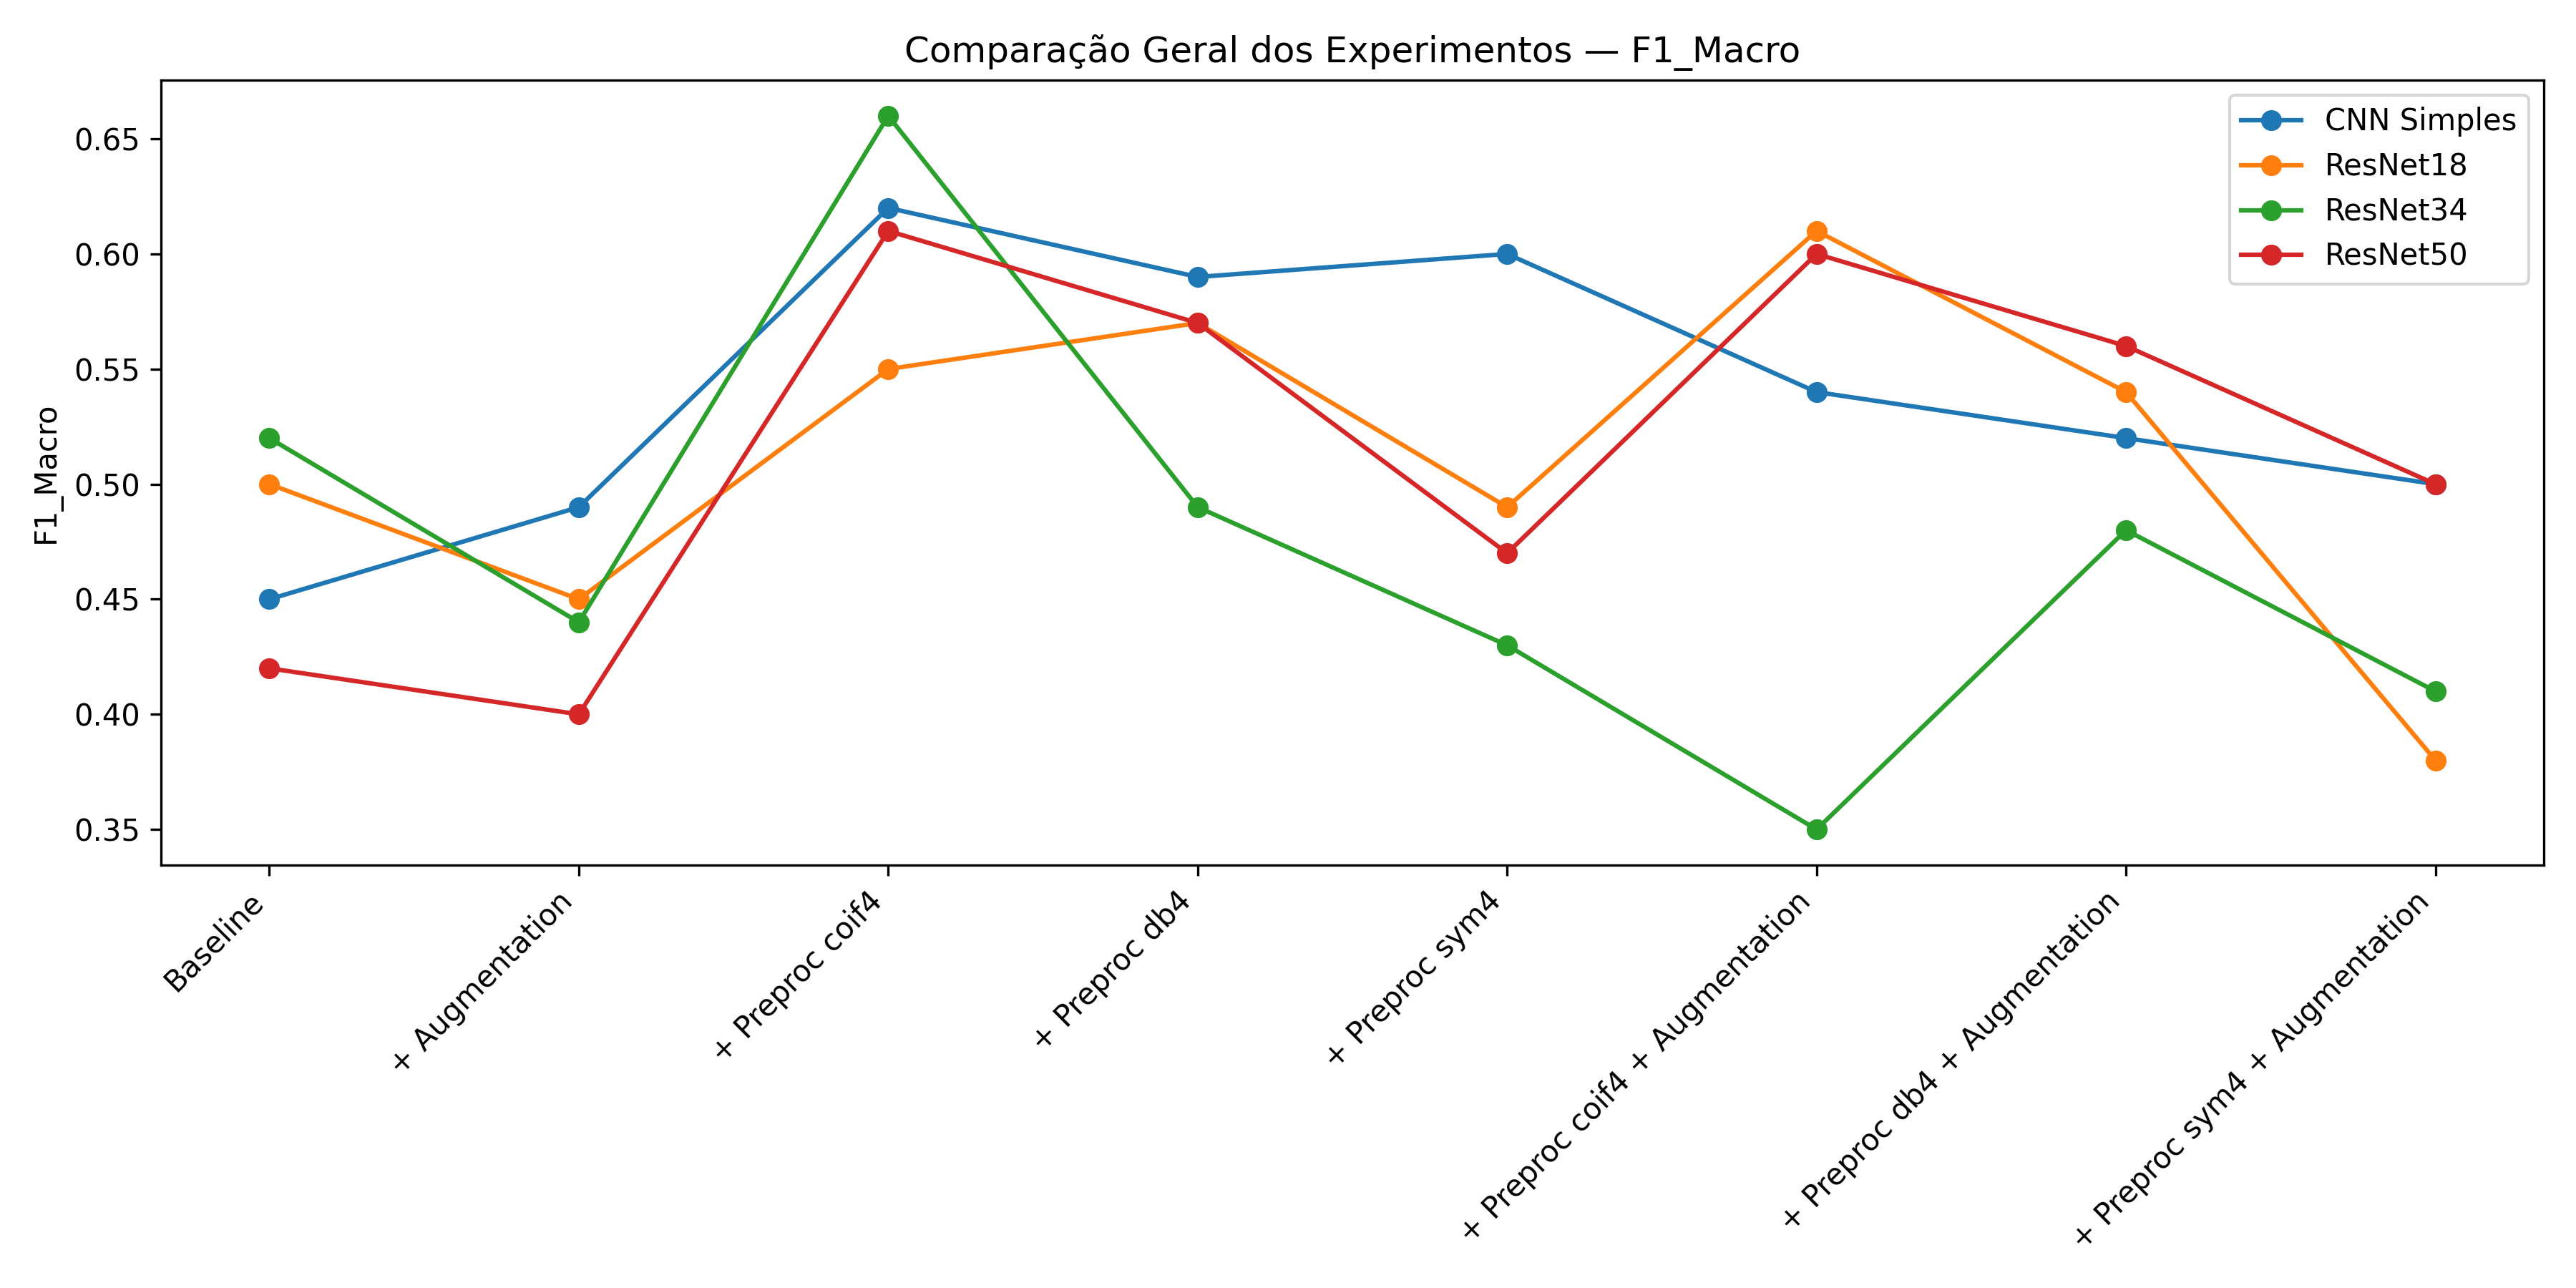
\includegraphics[width=\textwidth]{figuras/GERAL_F1_Macro.png}
    \label{fig:f1_macro}
    \fonteproprioautor
\end{figure}

\begin{figure}[!h]
    \caption{F1-score - Ponderado}
    \centering
    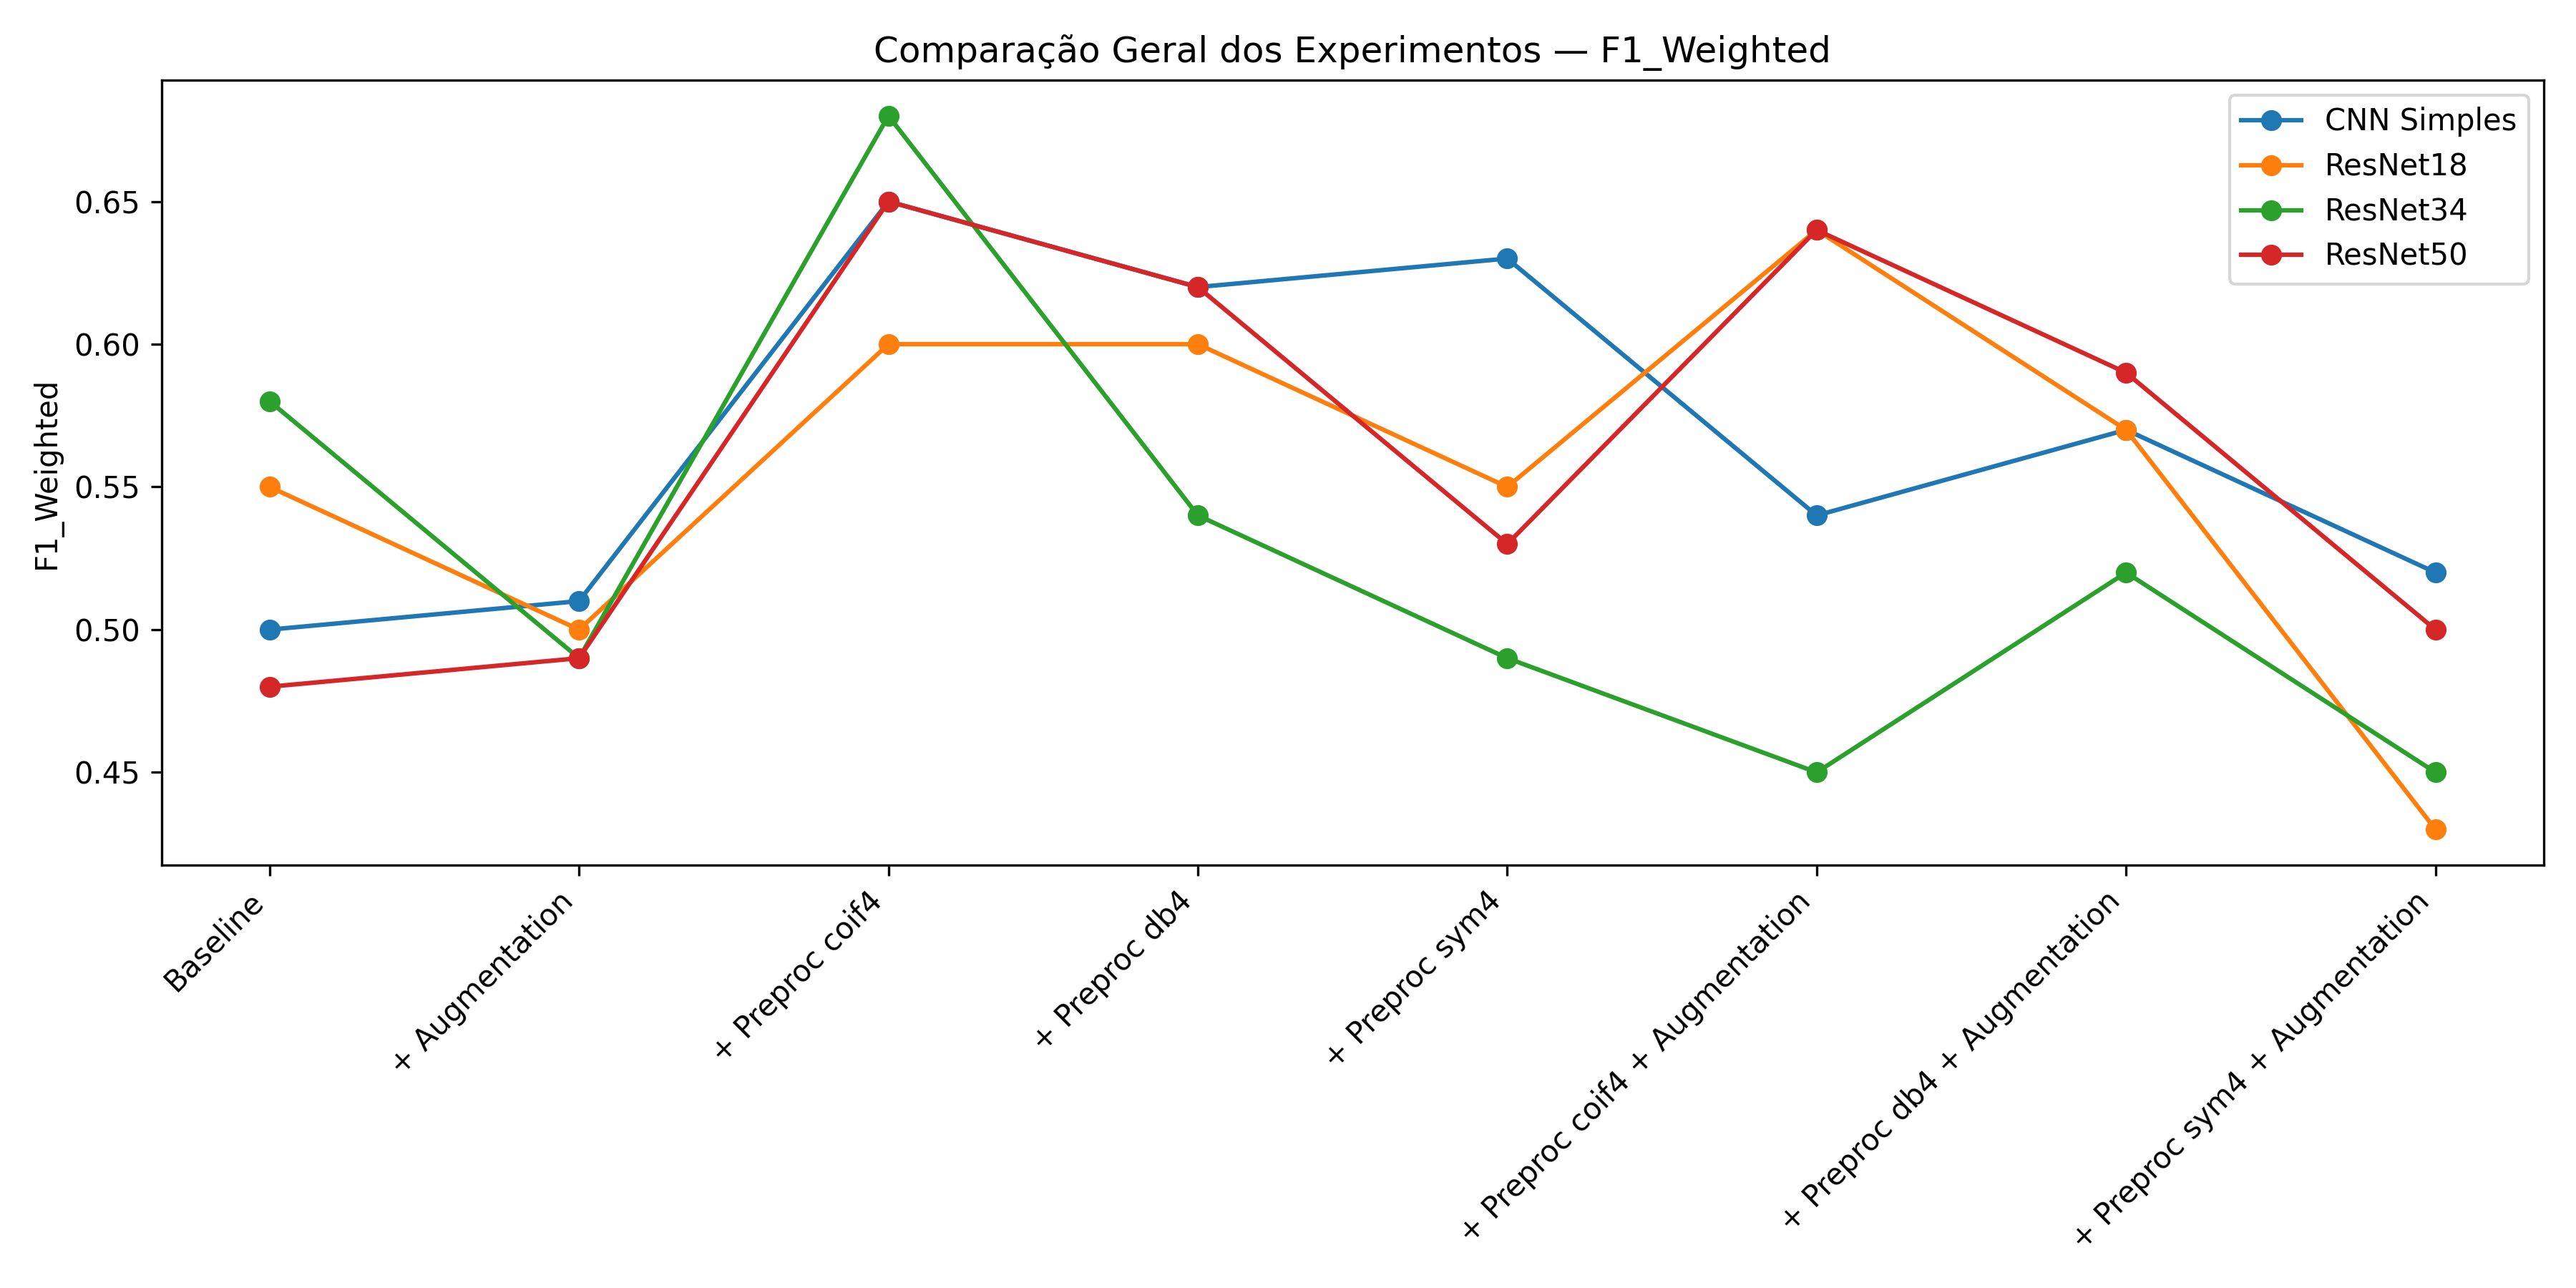
\includegraphics[width=\textwidth]{figuras/GERAL_F1_Weighted.png}
    \label{fig:f1_ponderado}
    \fonteproprioautor
\end{figure}

\begin{figure}[!h]
    \caption{Recall - Macro}
    \centering
    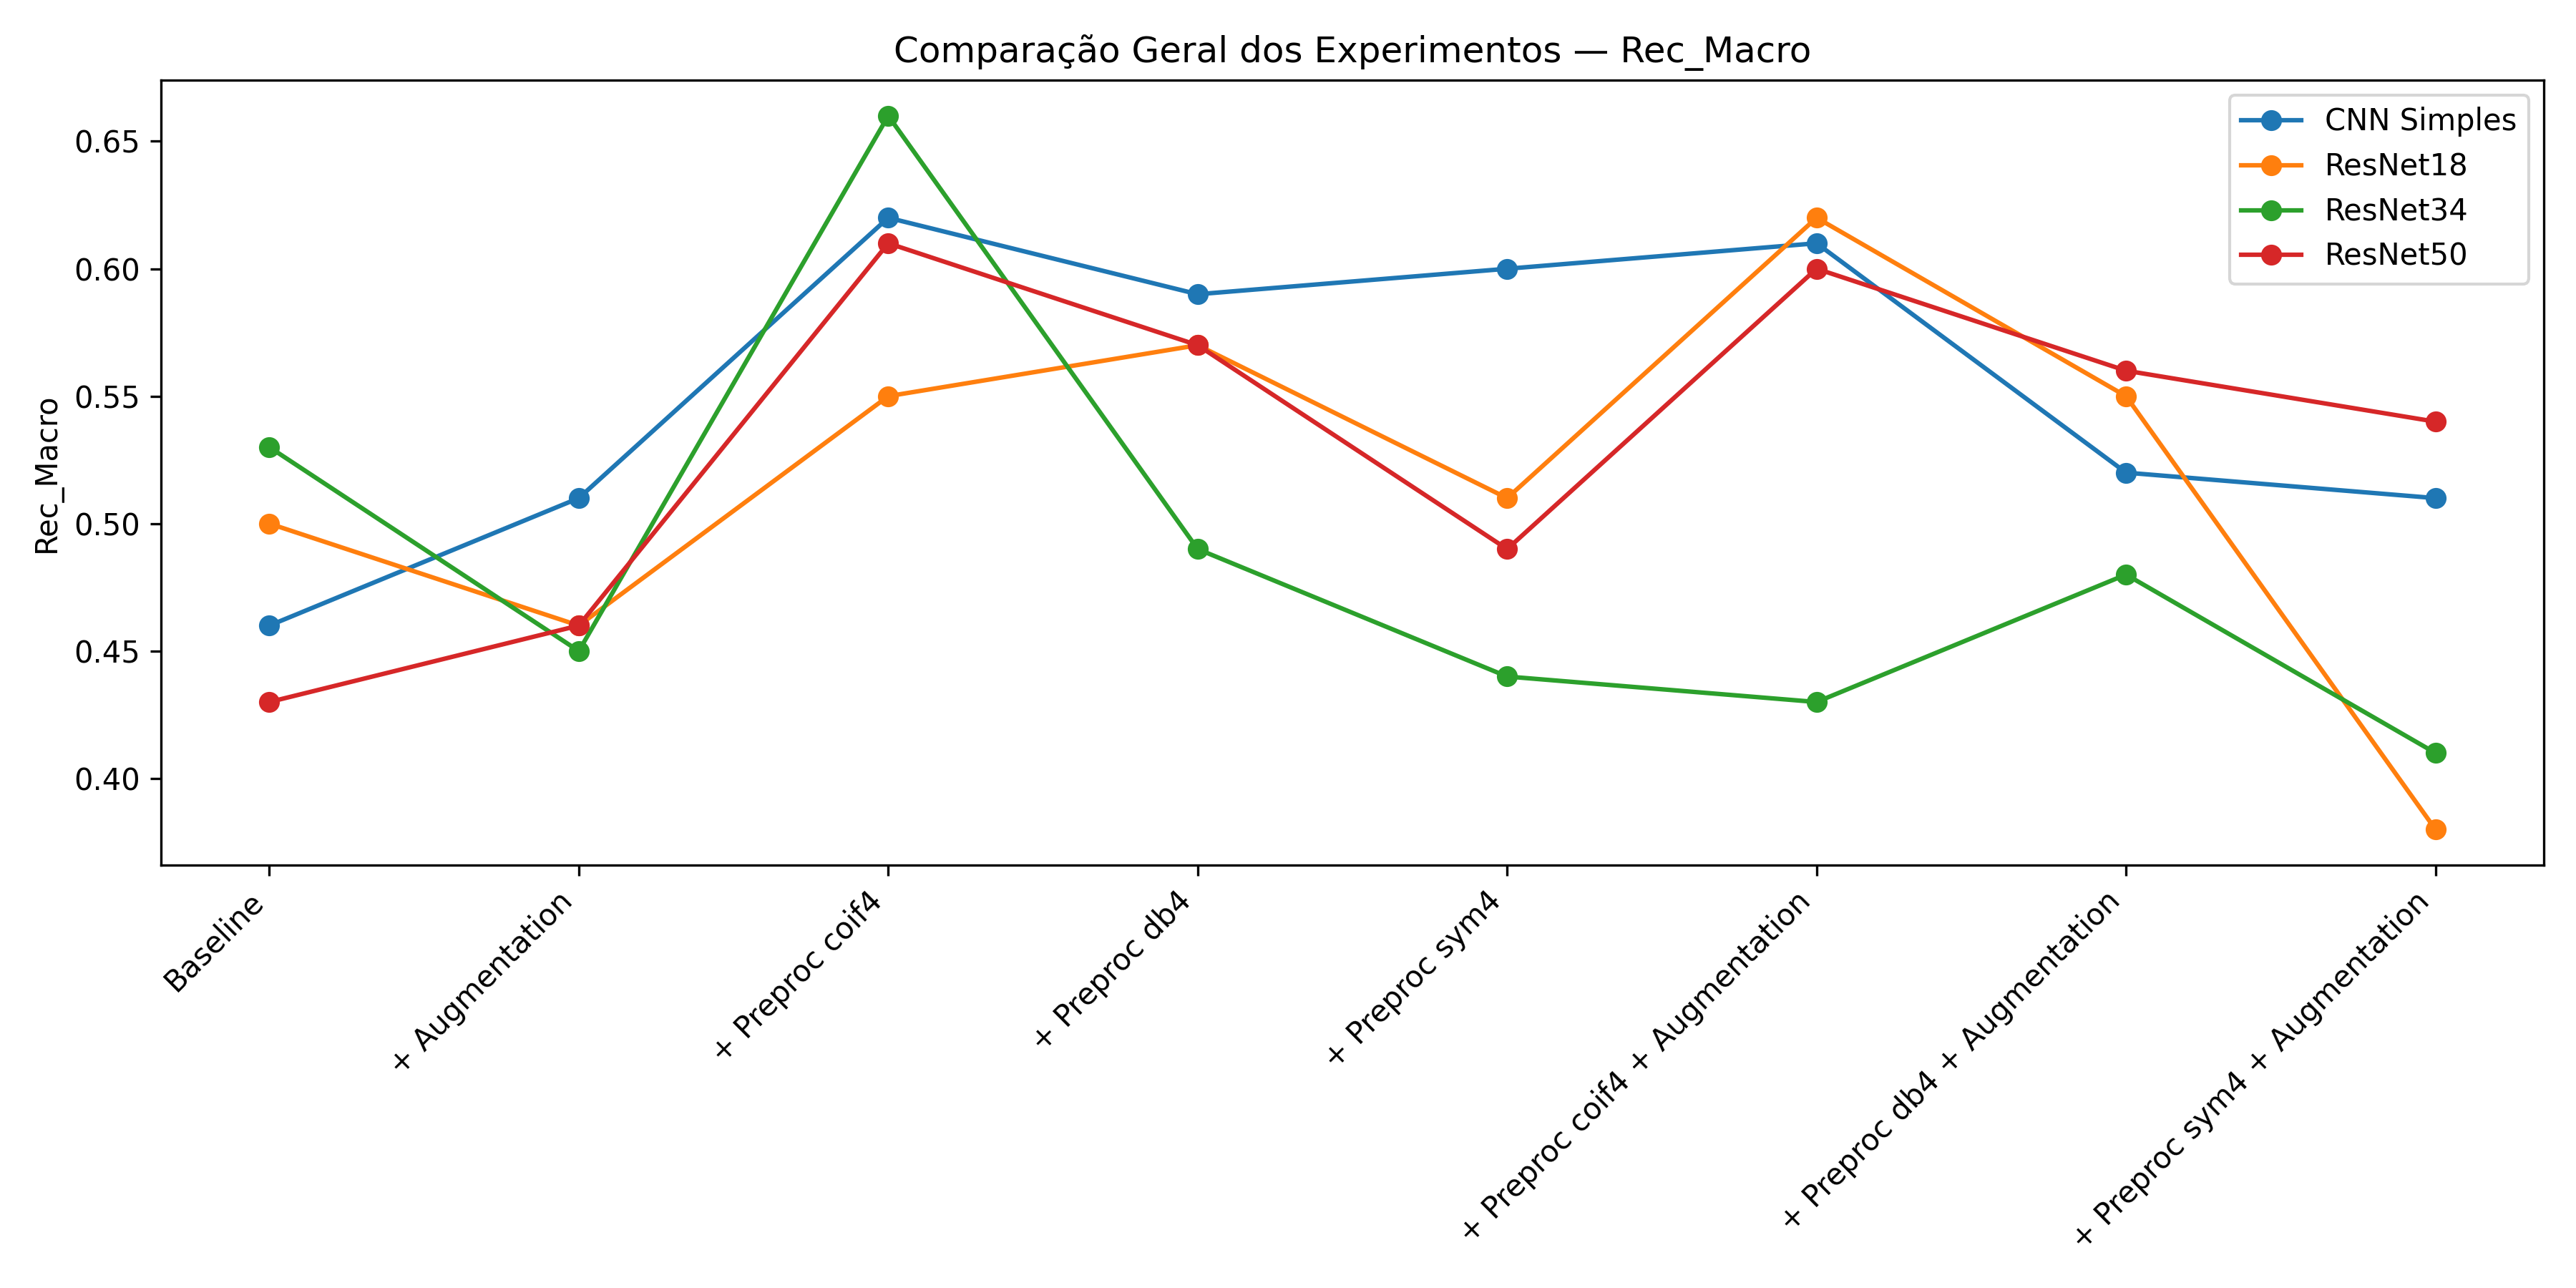
\includegraphics[width=\textwidth]{figuras/GERAL_Rec_Macro.png}
    \label{fig:recall_macro}
    \fonteproprioautor
\end{figure}

\begin{figure}[!h]
    \caption{Recall - Ponderado}
    \centering
    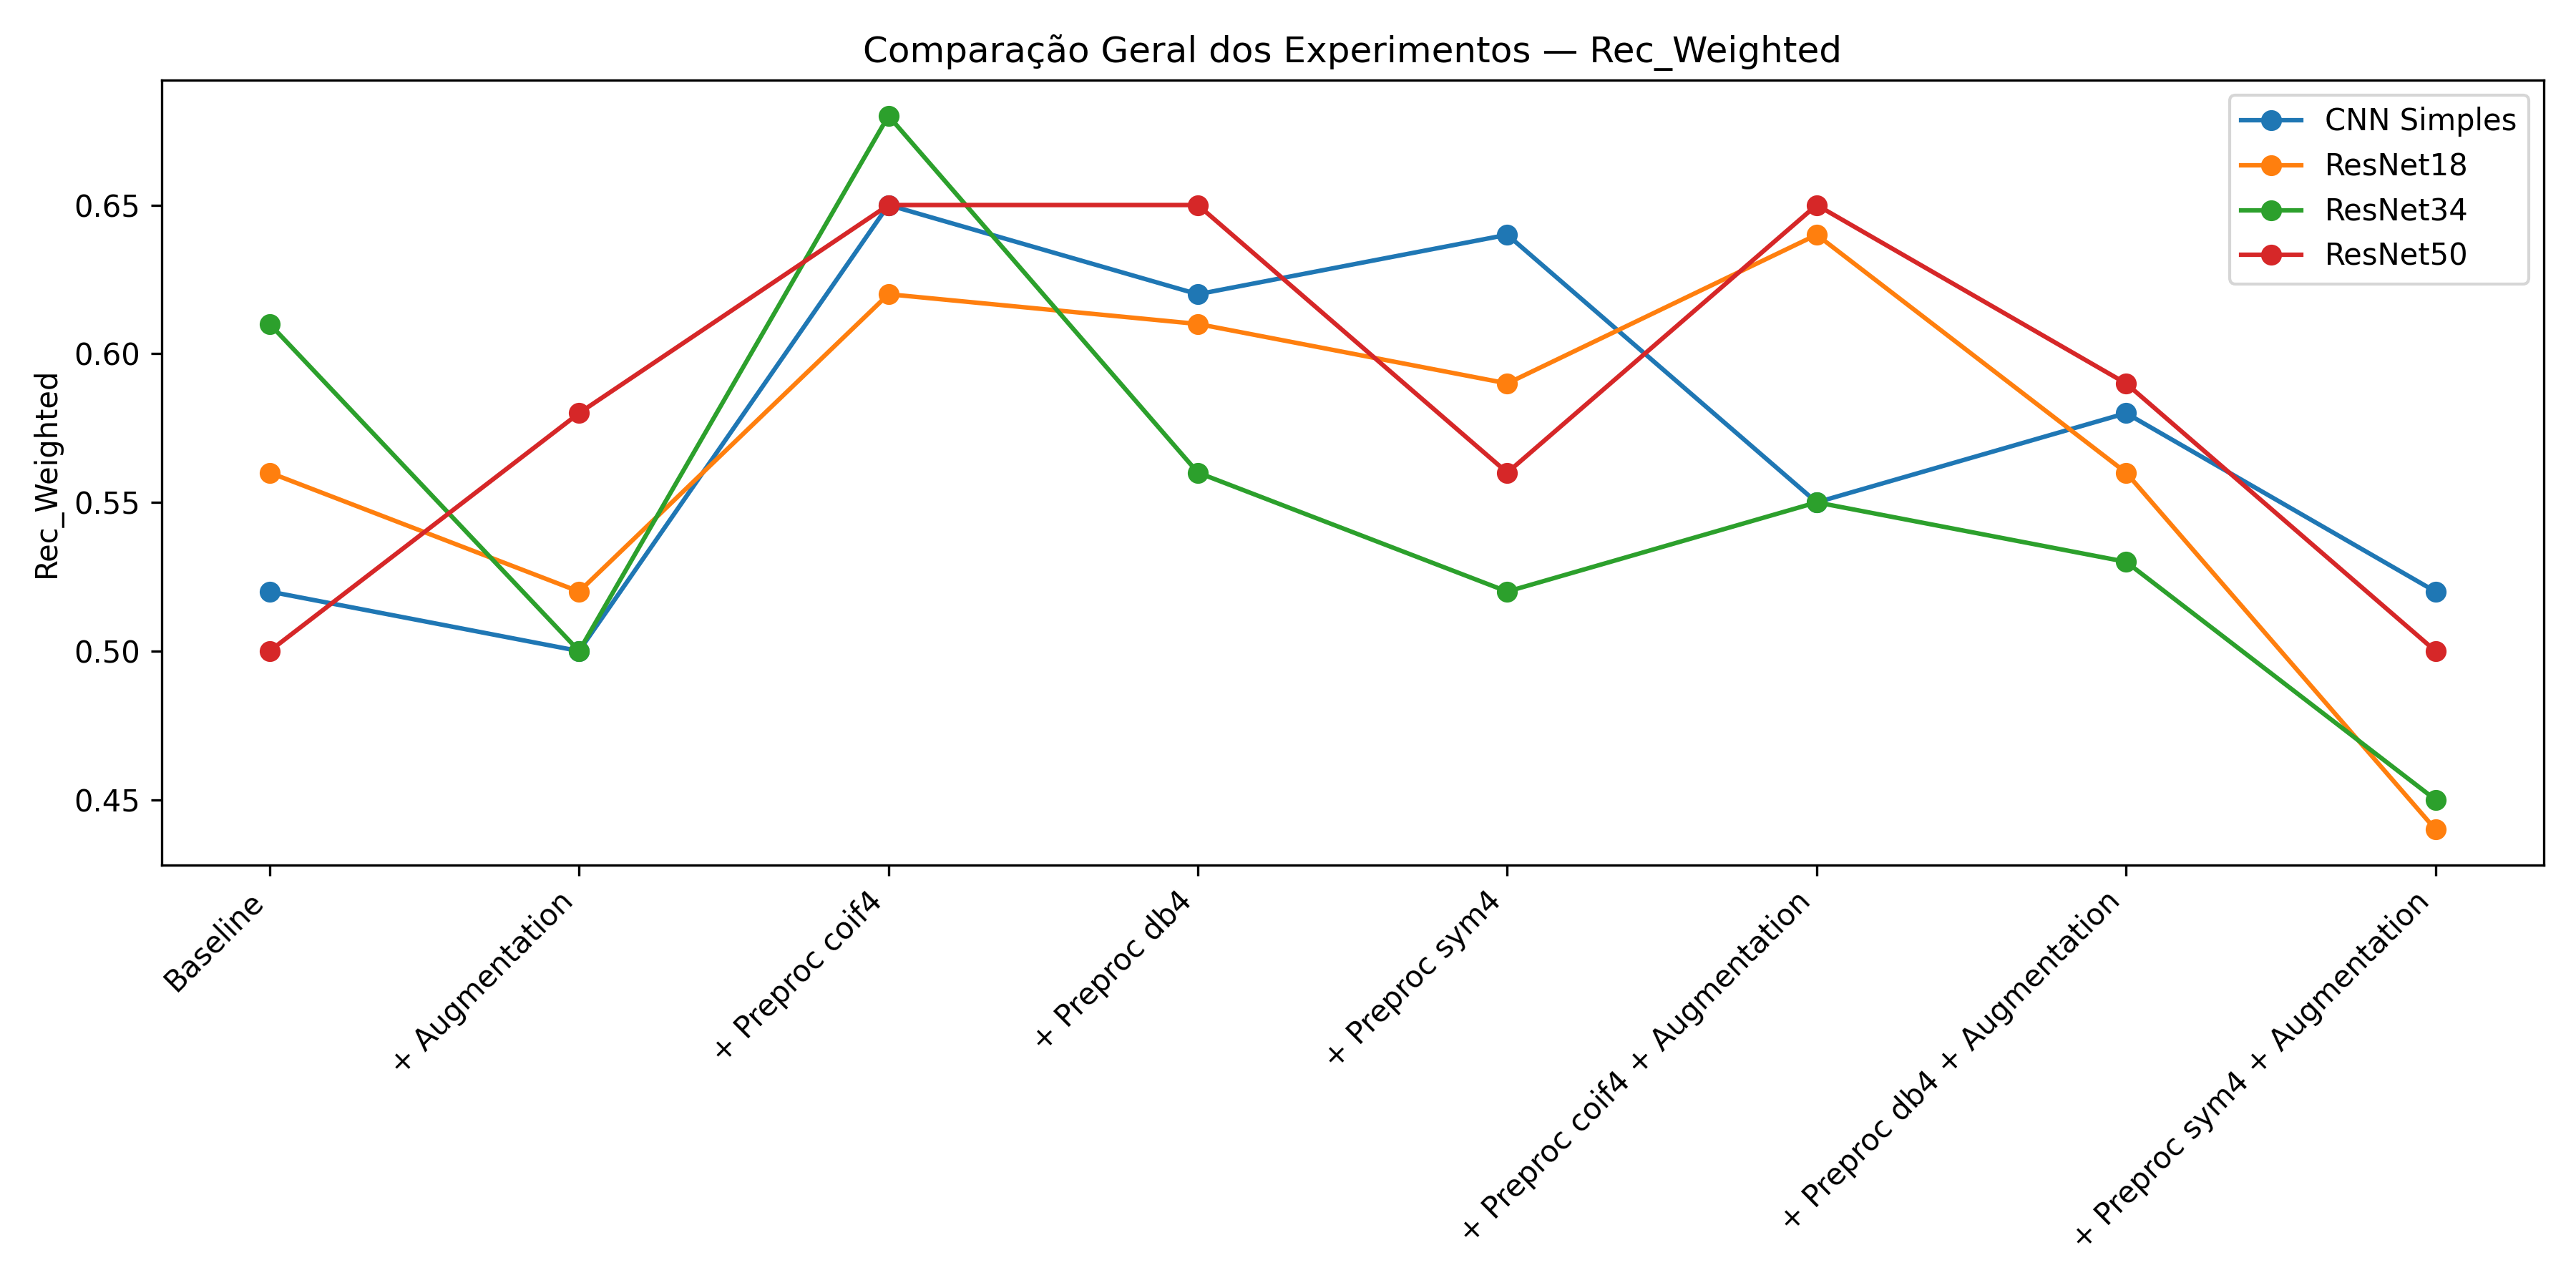
\includegraphics[width=\textwidth]{figuras/GERAL_Rec_Weighted.png}
    \label{fig:recall_ponderado}
    \fonteproprioautor
\end{figure}

\begin{figure}[!h]
    \caption{Precisão - Macro.}
    \centering
    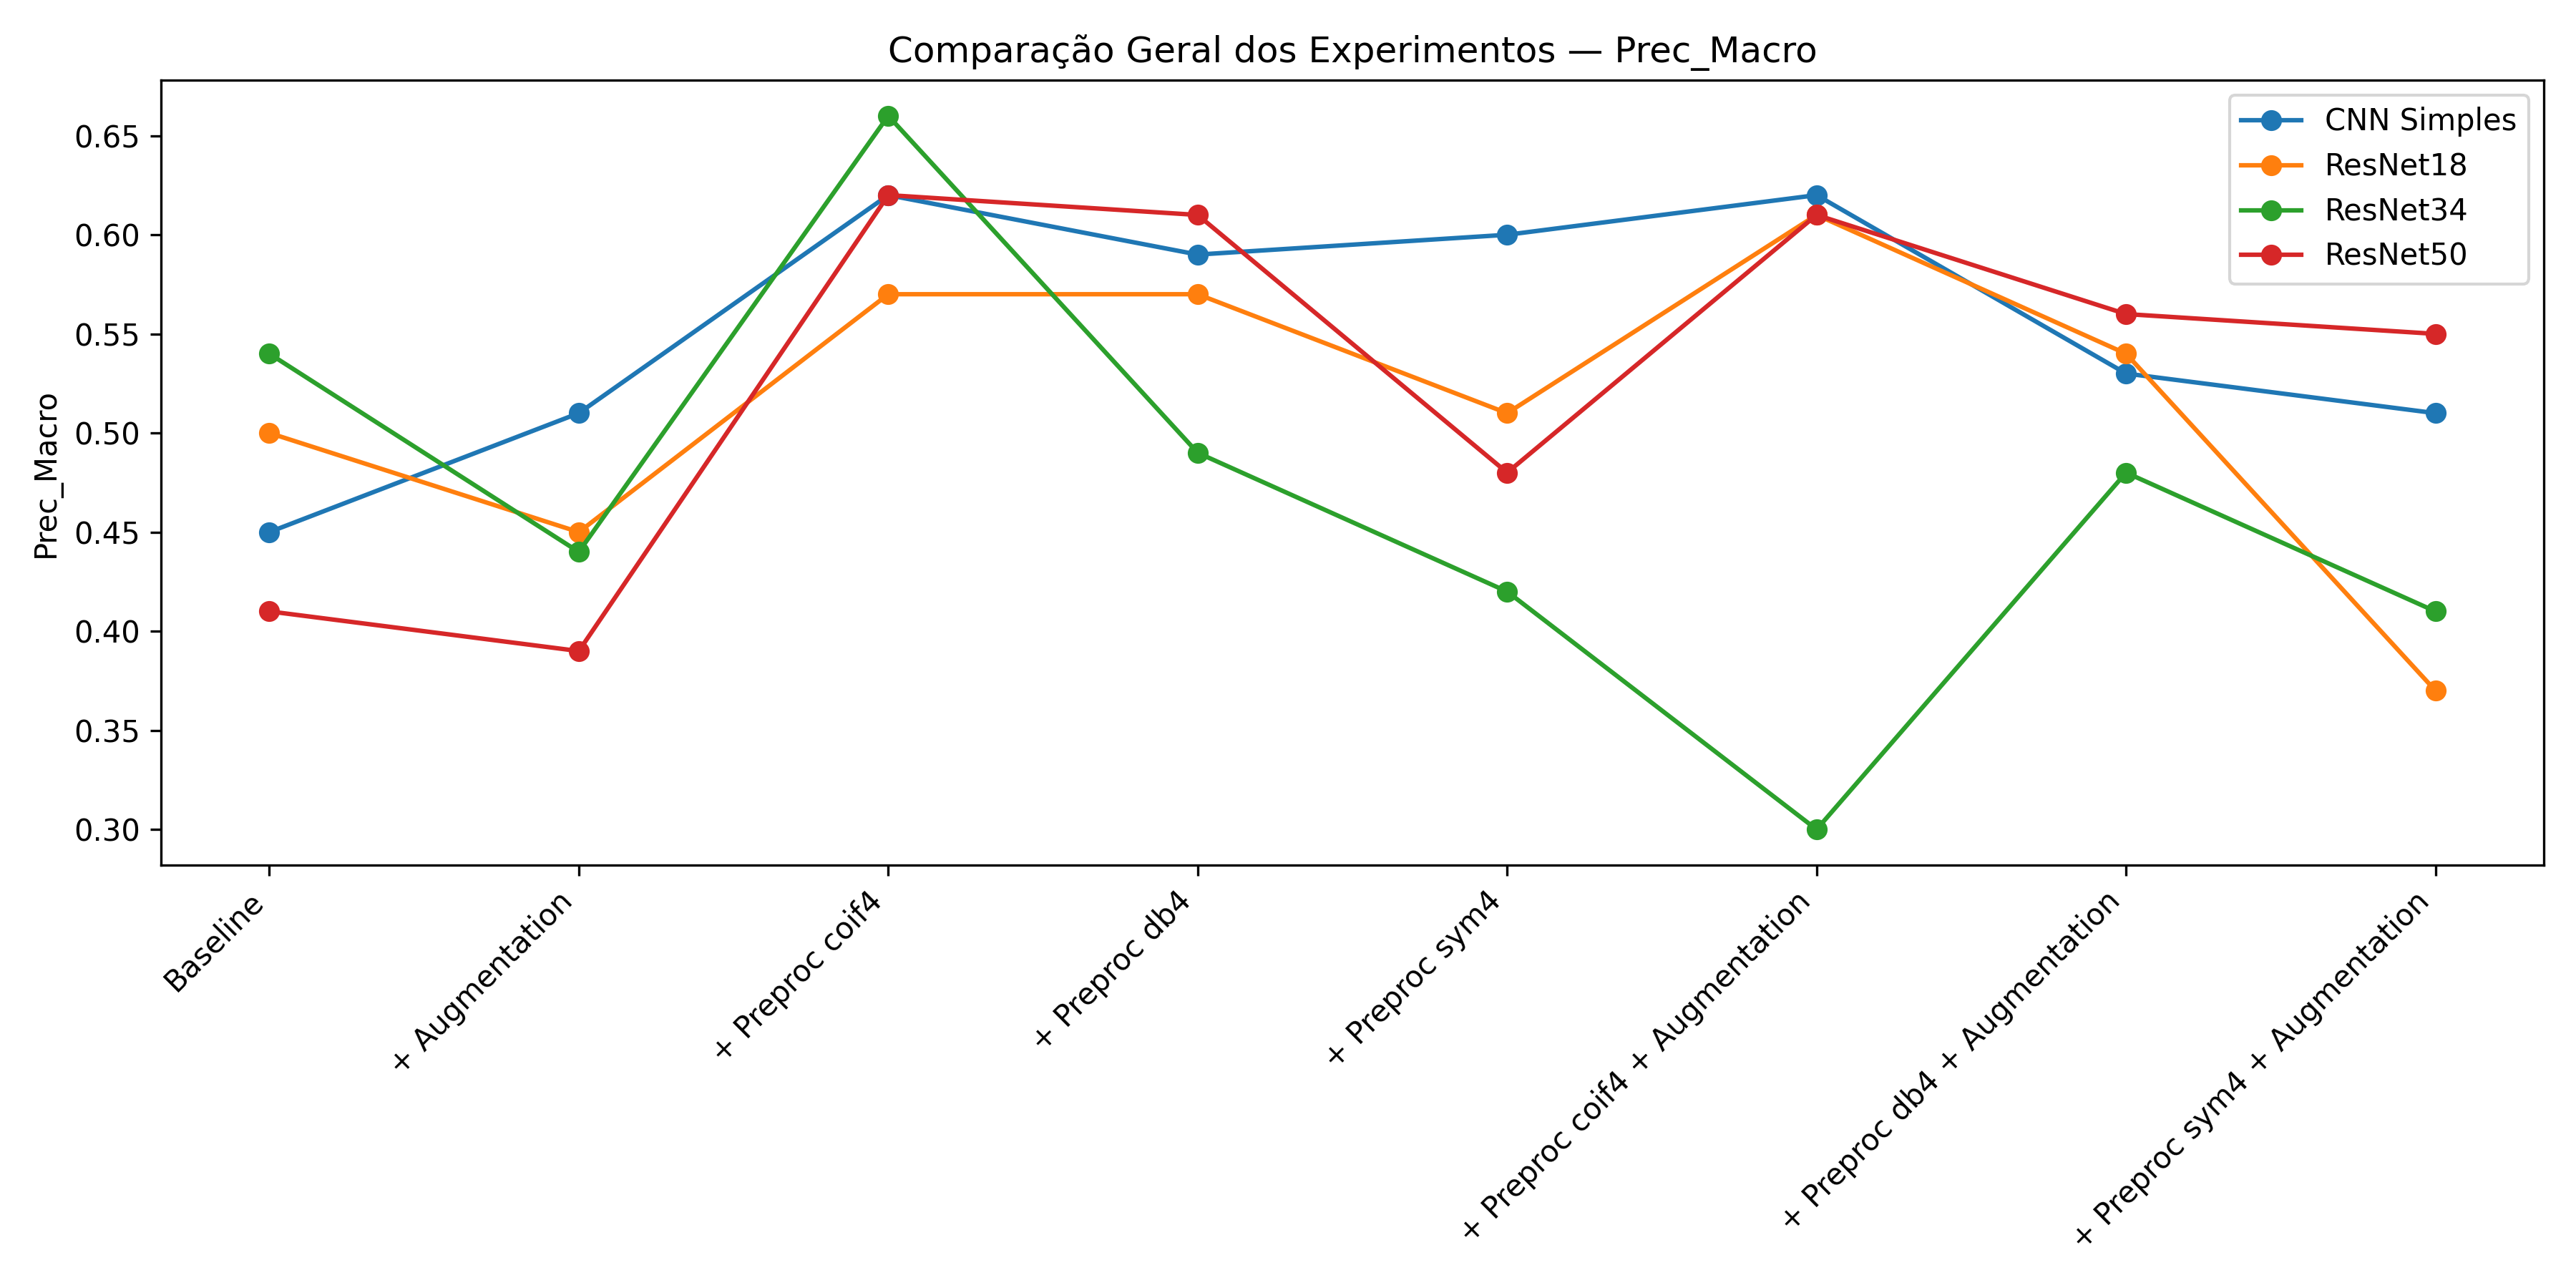
\includegraphics[width=\textwidth]{figuras/GERAL_Prec_Macro.png}
    \label{fig:prec_macro}
    \fonteproprioautor
\end{figure}

\begin{figure}[!h]
    \caption{Precisão - Ponderado}
    \centering
    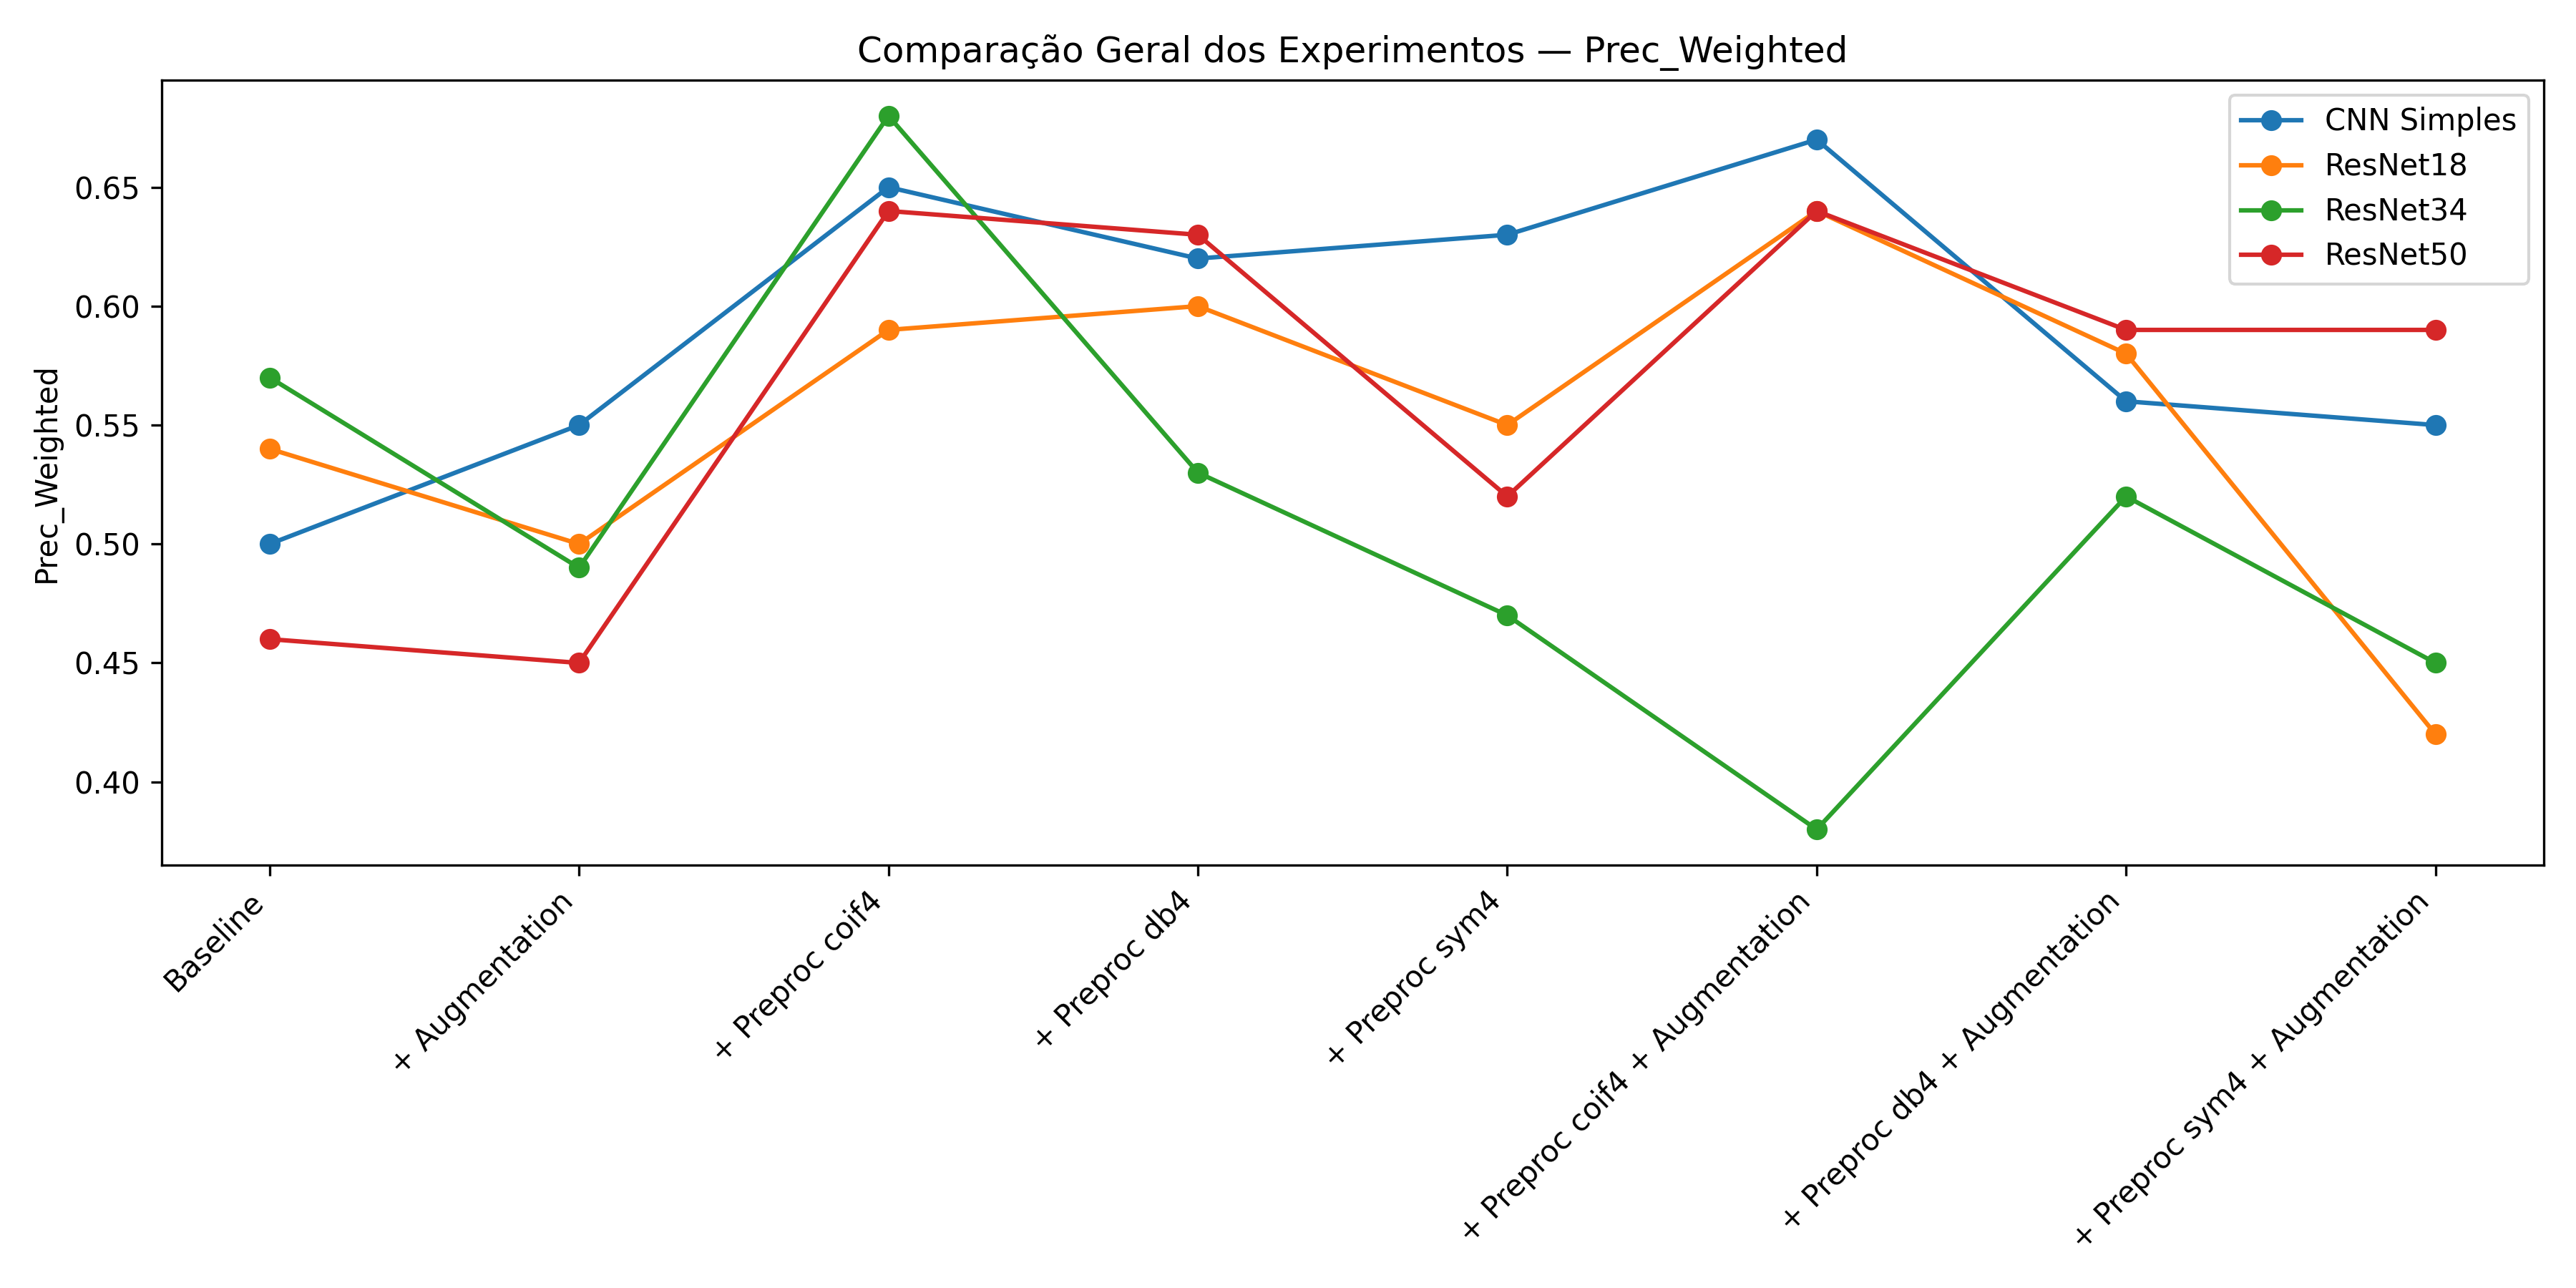
\includegraphics[width=\textwidth]{figuras/GERAL_Prec_Weighted.png}
    \label{fig:prec_ponderado}
    \fonteproprioautor
\end{figure}


\end{apendicesenv}
